\subsection{Brainstorm}
Ved projektets spæde opstart, fandt vi en stabel papir. Herefter skrev vi bud på spil, vi kunne lave ud fra de givne opgaveoplæg. Ideerne vi synes var uinteressante bortkastede vi samt de korresponderende oplæg. Vi nåede ad første omgang frem til, at det oplæg, som vi fandt mest interessant, var oplæg nr. 2.

Sidenhen kom vi med to bud på spil, vi kunne lave. Et vertical-scroller spil, hvor man stikker plastik med spyd og fjerne det fra en flod. Spillet skulle have store sorte bar på computer, således at billedhøjden bliver meget høj ift. billedbredden. Et andet spil, som vi gik med, jf. vores elevatorpitch, se \autoref{par:elevator_pitch}, var et top-down fixed-shooter spil, hvor monstre opstår som følge af skraldklynger. Papirerne er desværre gået tabt, ellers var de blevet vedhæftet som bilag.

\subsection{Flow}
Før vi begynder med den konkrete udvikling af spillet, er det vigtigt, helt strukturelt, at vi opbygger spillet med flow--teorien\footfullcite{flow} i tankerne. Flow--teorien beskriver, hvordan en spiller bedst bliver underholdt når han spiller et computerspil.
Hvis ens computerspil for hurtigt viser en meget høj sværhedsgrad, så giver det spilleren en angstlig følelse, hvilke virker negativt på hans lyst til at fortsætte med at spille spillet, og det er ikke hensigtsmæssigt. Hvis spillet derimod er af en lav sværhedsgrad og spillerens kompetenceniveau er for stort, vil spilleren kede sig og afbryde spillet. Hensigten er derfor at skabe et spil som gradvist øger sværhedsgraden sideløbende med at spillerens kompetencer forøges, eksempelvis ved at lave forskellige sværhedsgrader, så forskellige niveauer af kompetencer akkommoderes.

\begin{figure}[H]
    \centering
    \fbox{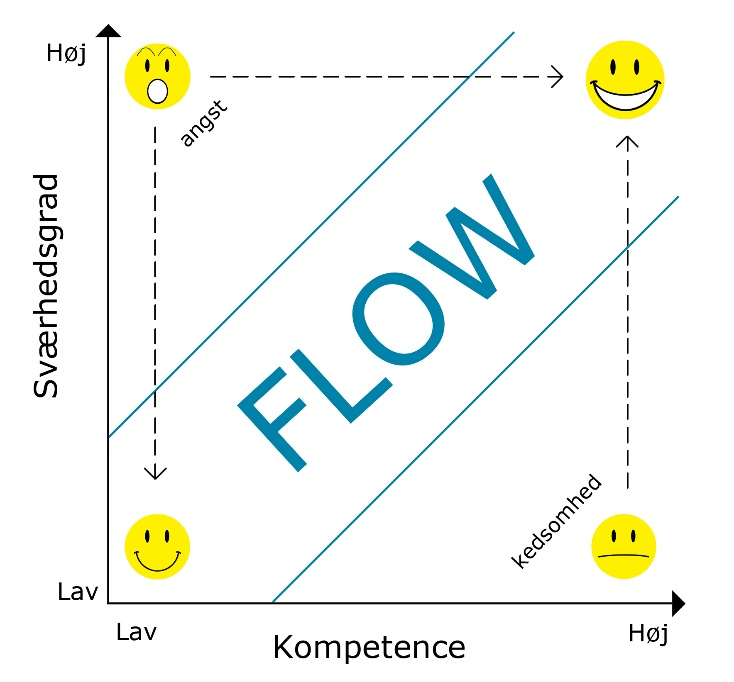
\includegraphics[width=0.5\linewidth]{assets/flow.jpg}}
    \caption{Viser flowstadiet. Kilde: \cite{flow_chart}}
\end{figure}

Som vi beksriver senere i rapporten, bliver spillet på et tidspunkt udgivet i en Early Access udgave jf. \autoref{sec:udviklingsstadie}, her vil vi få en større spillerbase og teste flow på. Vi har derfor en masse konstanter (de er konstanter i den programmeringsmæssige forstand, konstante i de endelige binærer. De kan selvfølgelige ændres inden kompilering) i spillet som vi i Early Access vil kunne skrue på for at opnå det optimale flow.

\subsection{Paper-dummy - test I}
Paper dummys er et værktøj, som bruges tidligt i udviklingsfasen af et computerspil. 
Paper dummys er groft sagt at omsætte en spillidé til et brætspil for at teste dets 
spilmekanikker. Det er en billig, hurtig og nem lavteknologisk metode, som giver os 
mulighed for hurtigt at afprøve og diskutere ideer, uden at have investeret mange timer 
i udviklingen af en del af spillet, som måske ender med at være dårlig.

Vi har benyttet paper dummy-metoden til at teste vores grundlæggende spilmekanikker, 
herunder bevægelse, skydning, opsamling, monster-spawning og skralde-spawning i 
sammenspil med havstrømmene. Som det fremgår af \autoref{fig:main}, blev et simpelt 
gitter tegnet på papir, og vi krøllede papirskugler sammen som plastikskraldssimulatorer. 
Vores testperson fik reglerne at vide, og testen gik i gang.

Undervejs i testen fandt vi ud af, at der var mange regler, vi ikke havde tænkt over, 
hvilket resulterede i, at testsubjektet blev meget frustreret, da vi blev nødt til at 
tilføje regler ad hoc.

Paper dummyen udmundende i at, inden den entlige spiludvikling startede, skulle vi have præciseret reglerne meget mere.


\begin{figure}[H]
    \centering
  % --- Row 1: three images ---
  \begin{subfigure}[t]{0.32\textwidth}
    \fbox{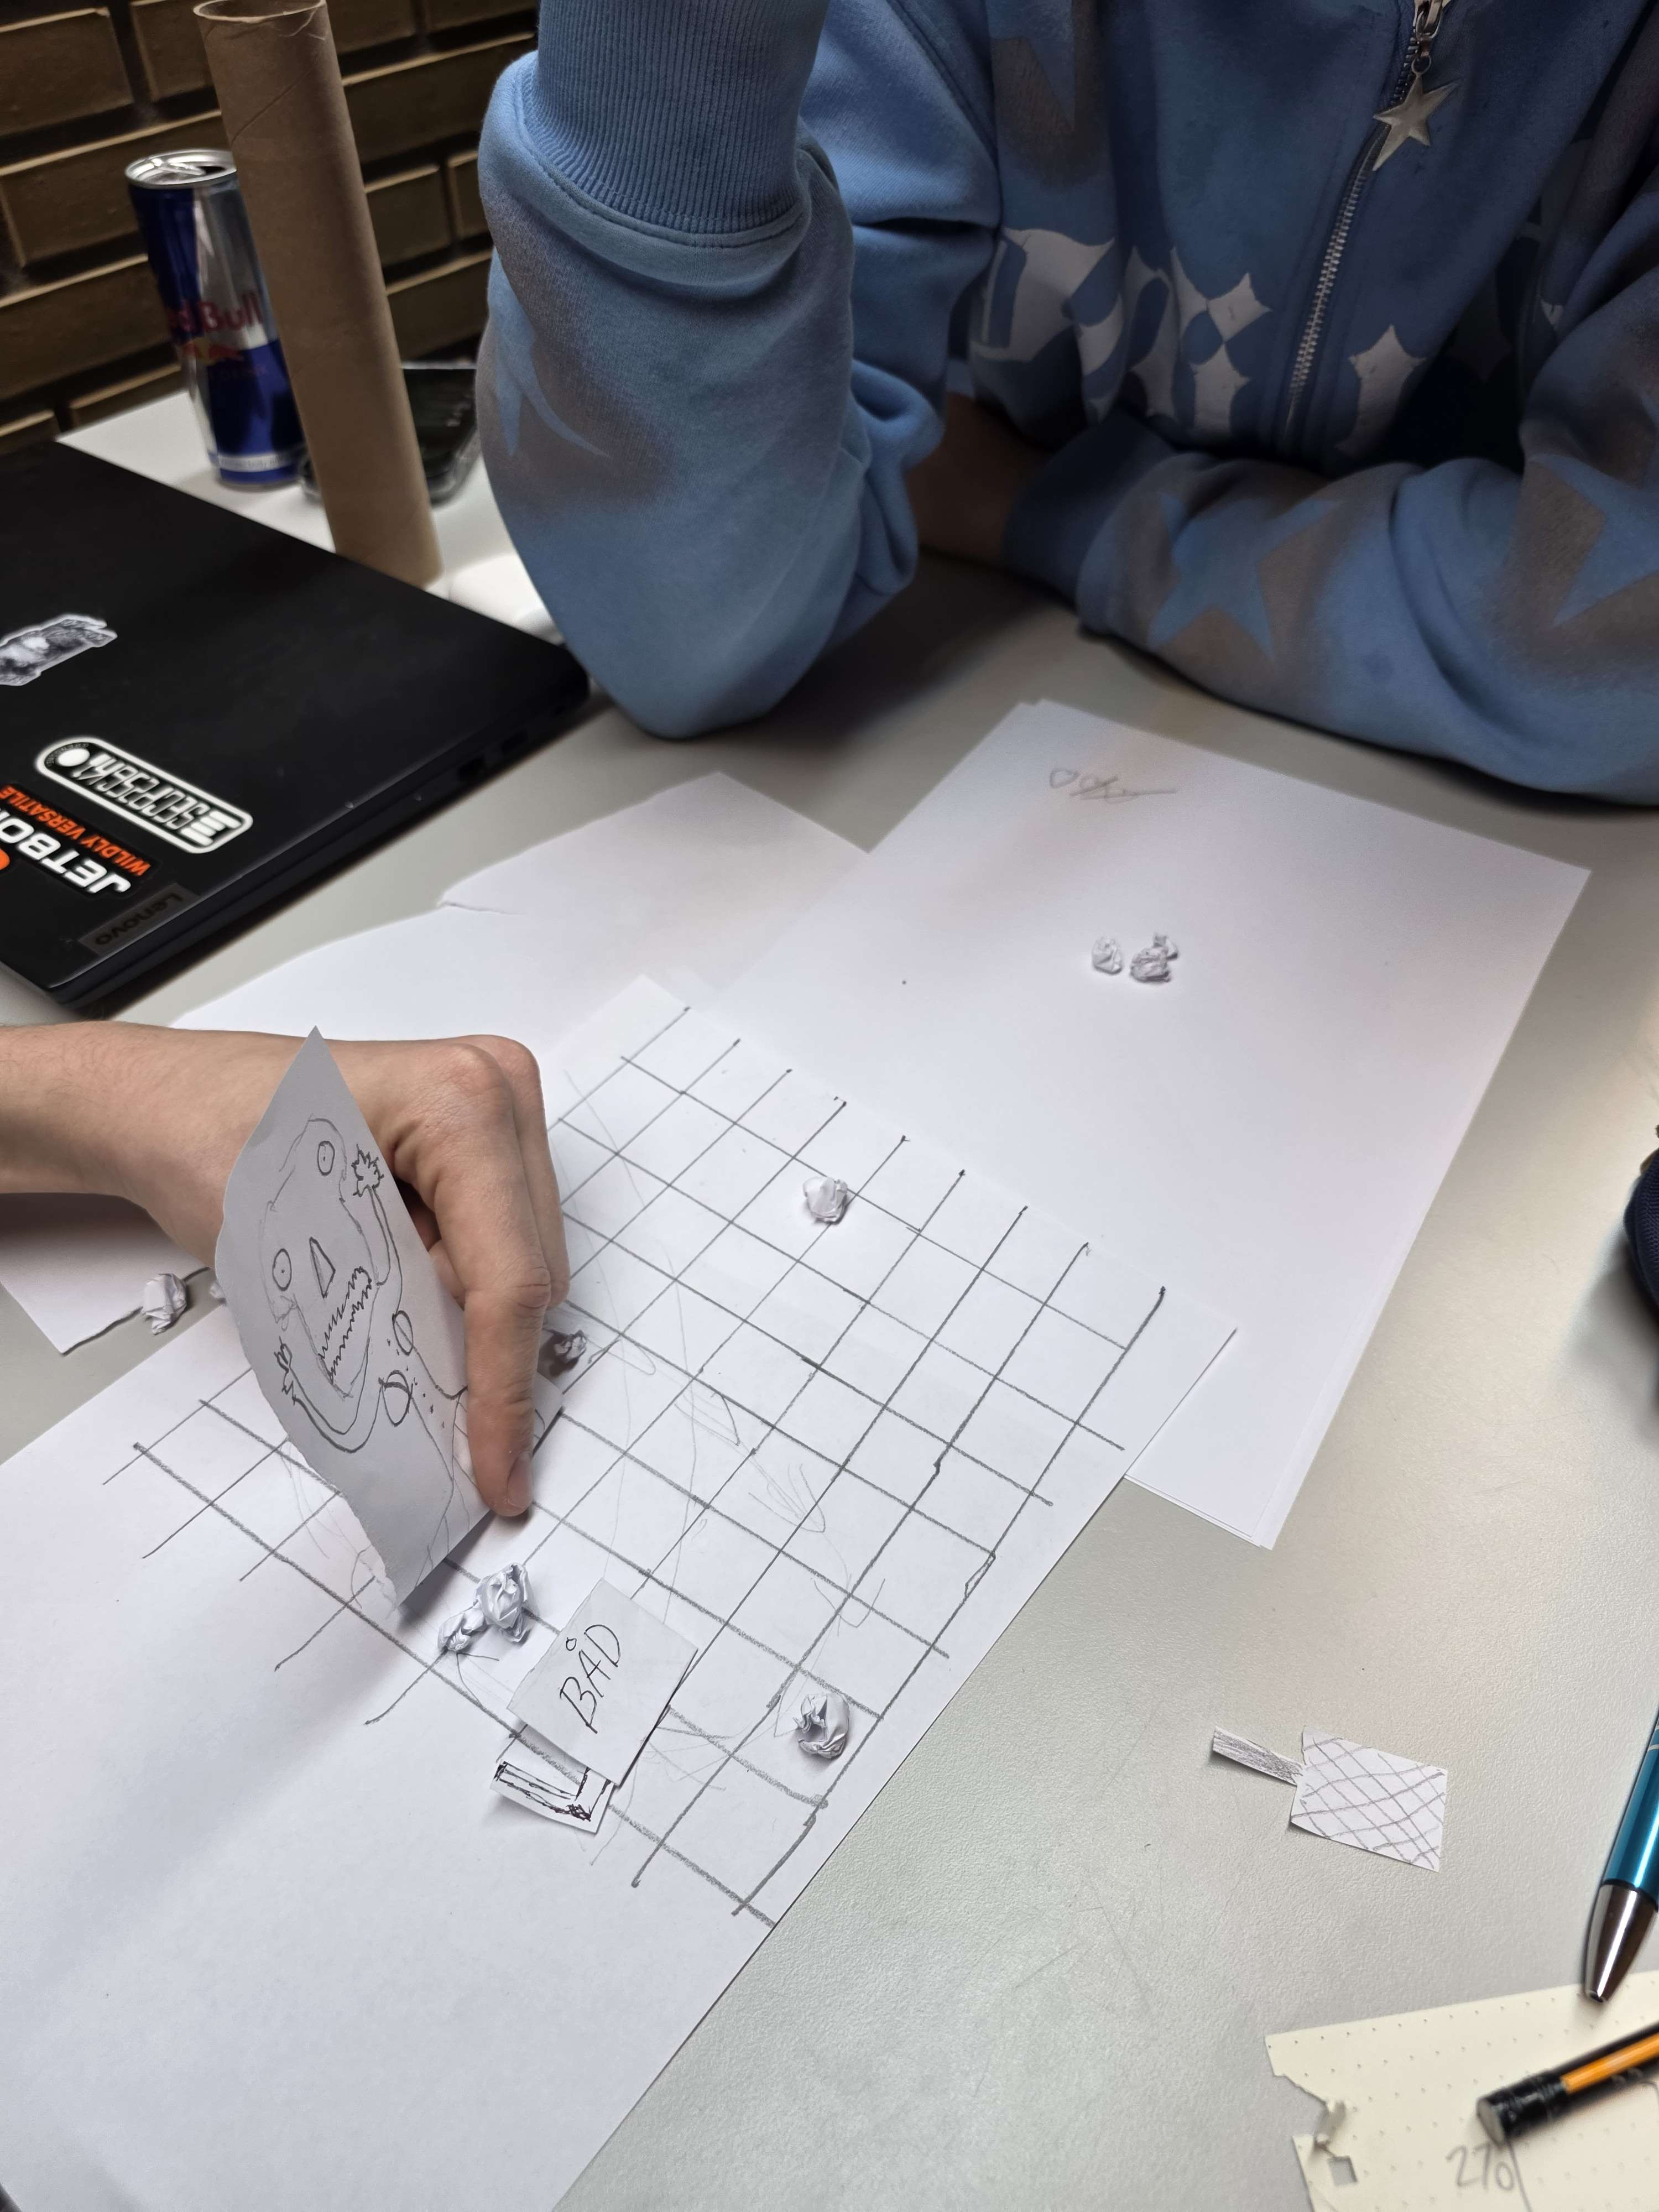
\includegraphics[width=\linewidth]{assets/paper_dummy_1.jpg}}
    % \caption{Caption a}
    \label{fig:a}
  \end{subfigure}
  \hfill
  \begin{subfigure}[t]{0.32\textwidth}
    \fbox{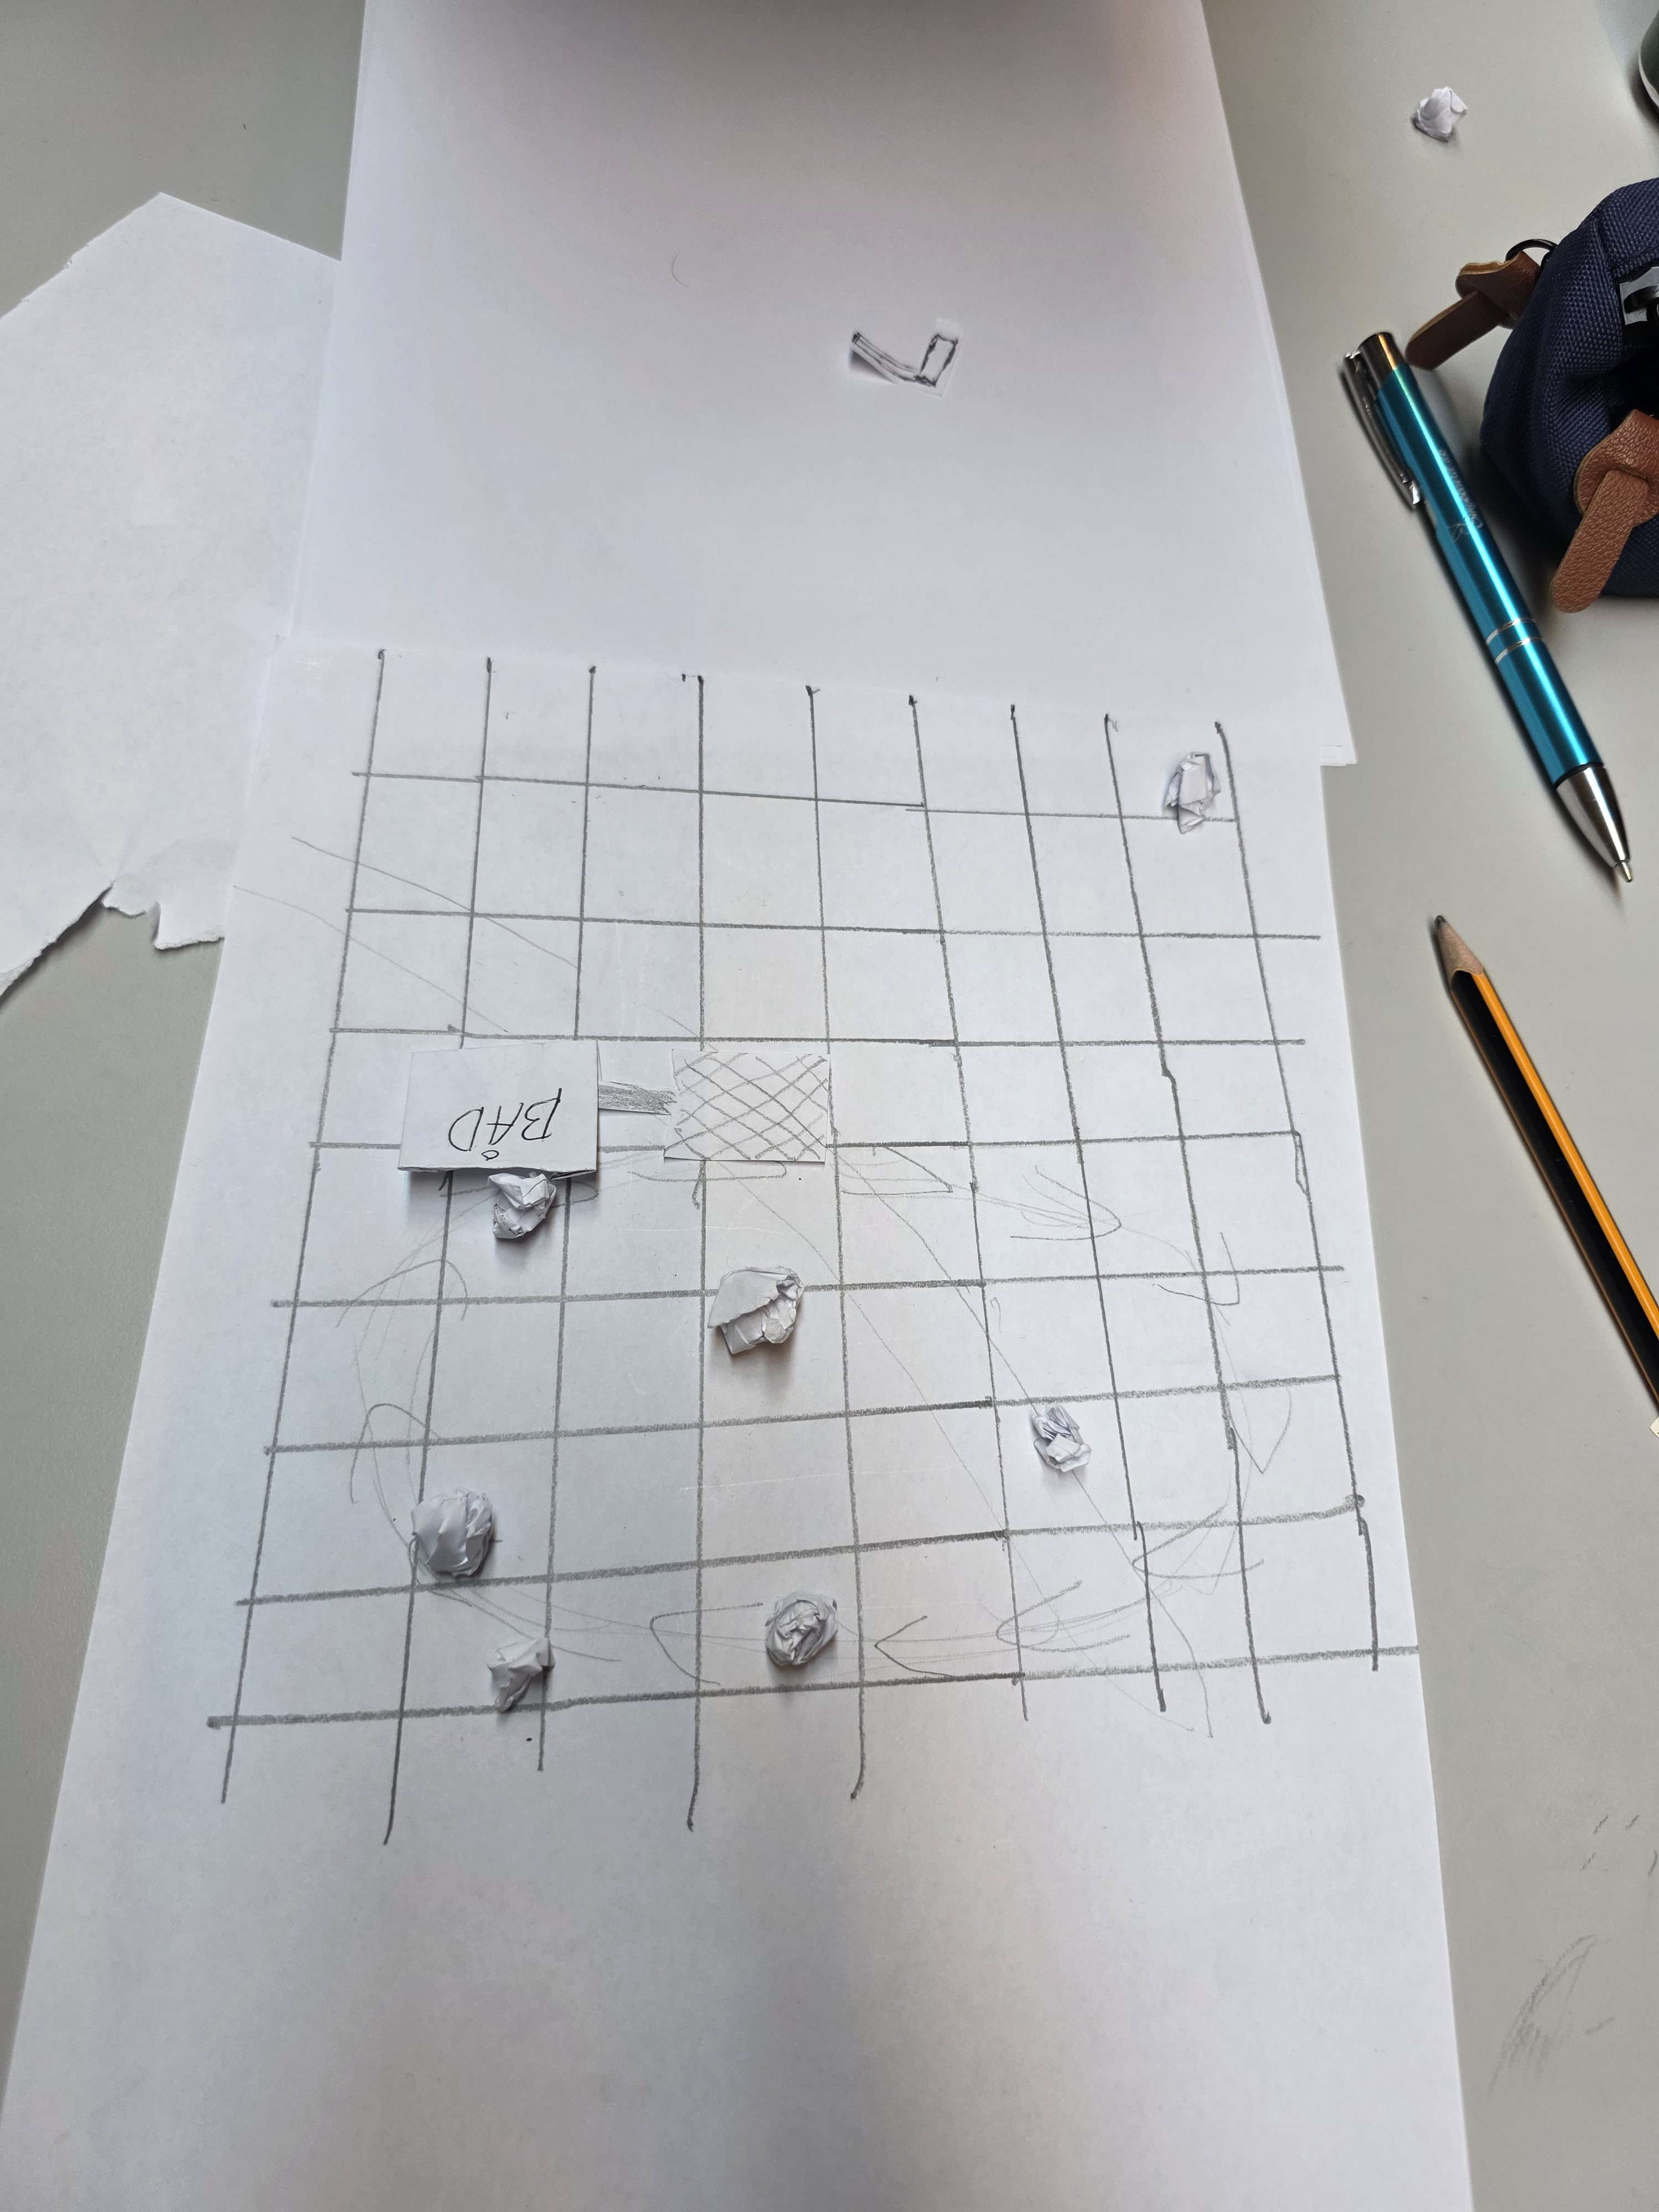
\includegraphics[width=\linewidth]{assets/paper_dummy_2.jpg}}
    % \caption{Caption b}
    \label{fig:b}
  \end{subfigure}
  \hfill
  \begin{subfigure}[t]{0.32\textwidth}
    \fbox{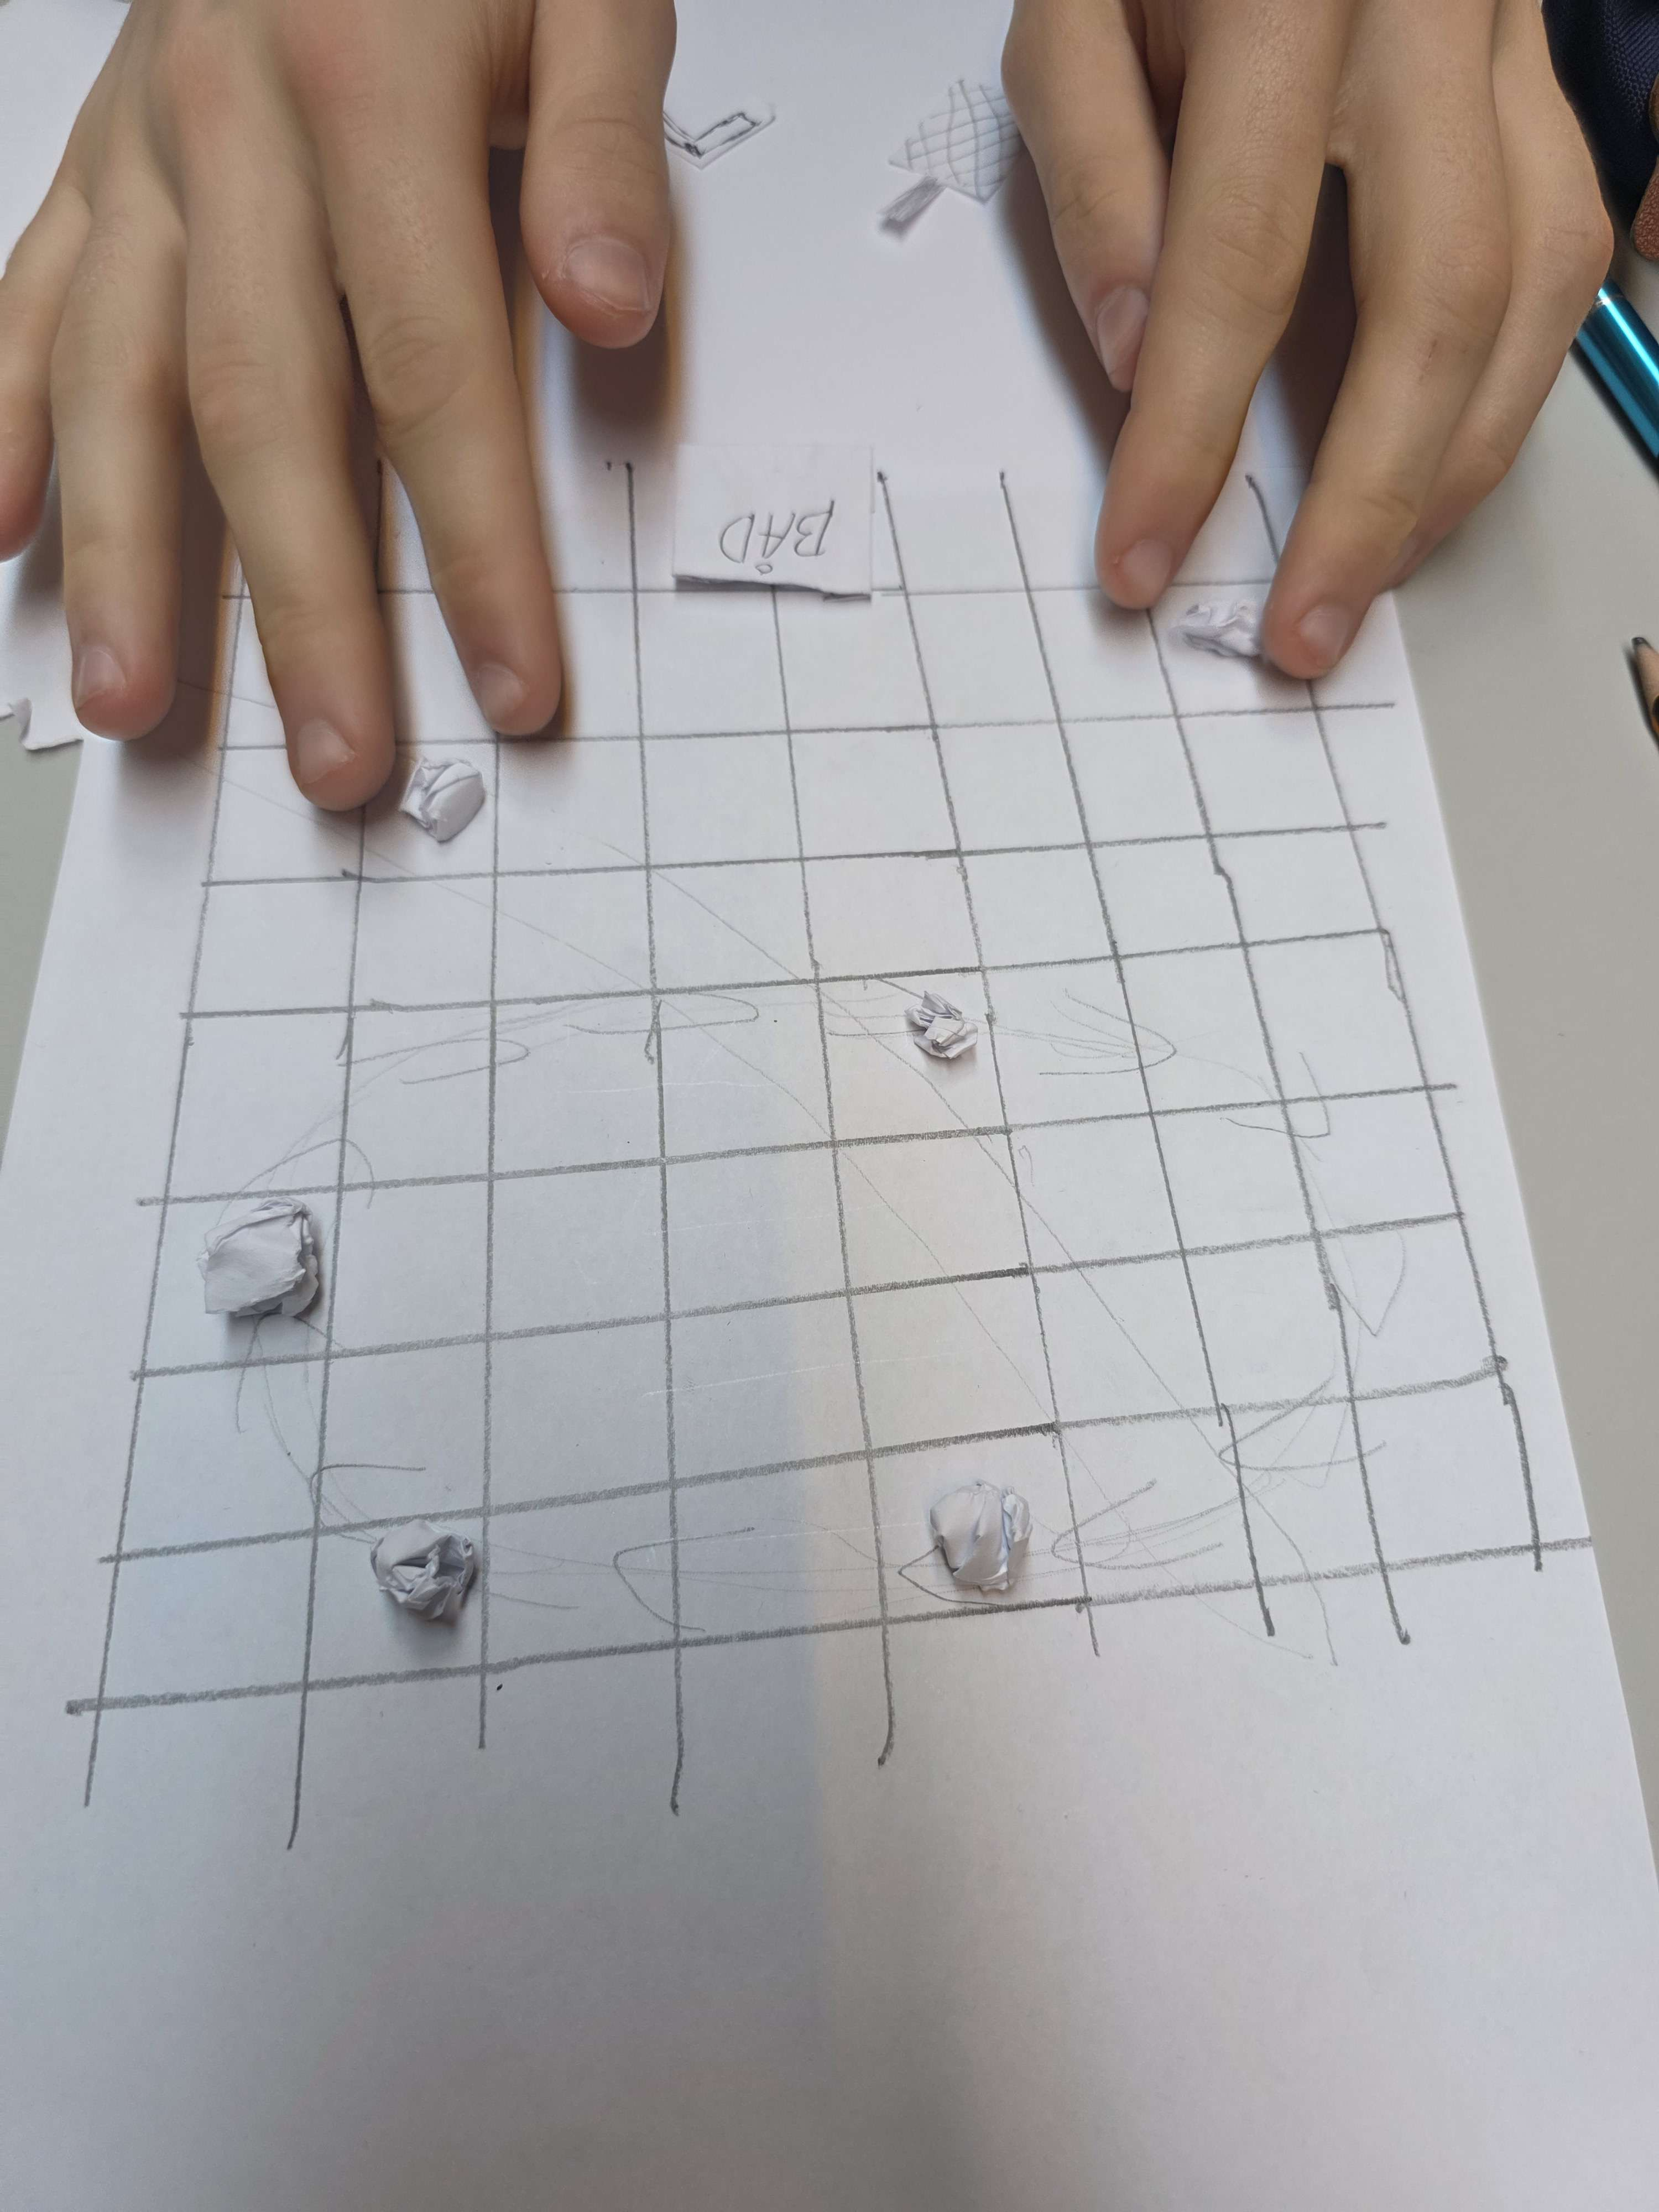
\includegraphics[width=\linewidth]{assets/paper_dummy_3.jpg}}
    % \caption{Caption c}
    \label{fig:c}
  \end{subfigure}

  \vspace{4pt} % small gap between rows

  % --- Row 2: two images centred ---
  \begin{subfigure}[t]{0.32\textwidth}
    \fbox{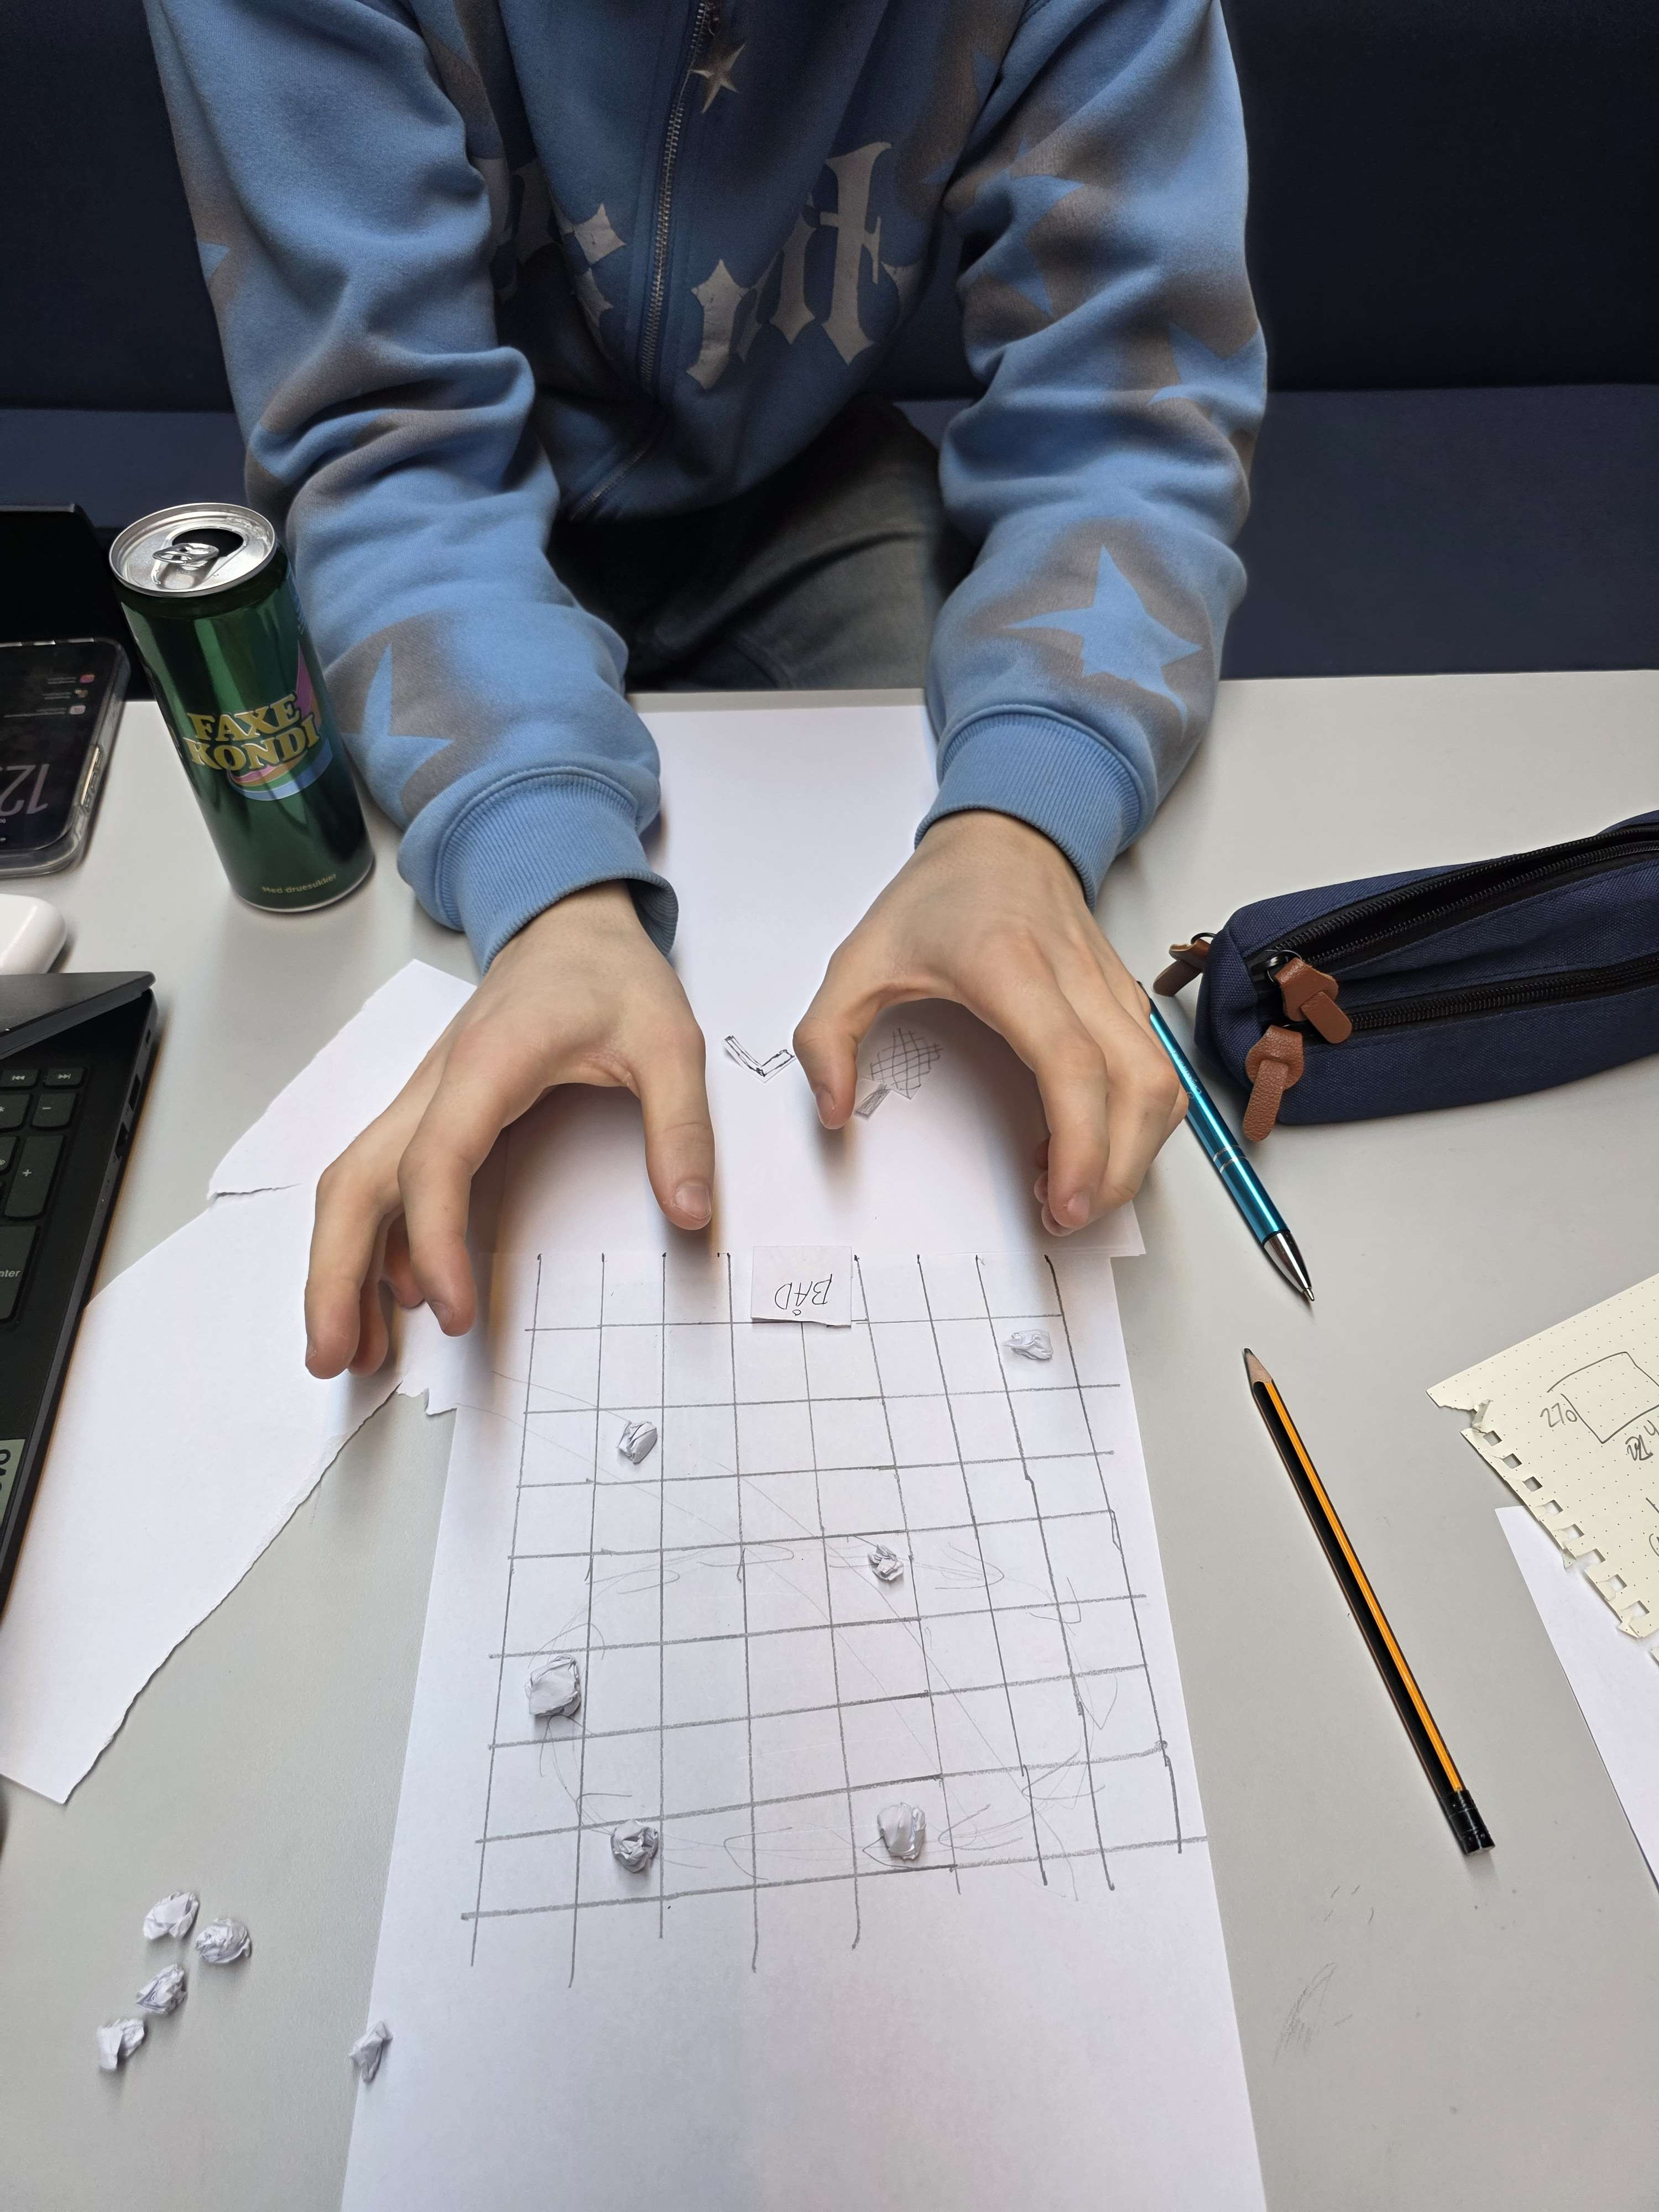
\includegraphics[width=\linewidth]{assets/paper_dummy_4.jpg}}
    % \caption{Caption d}
    \label{fig:d}
  \end{subfigure}
  \hfill
  \begin{subfigure}[t]{0.32\textwidth}
    \fbox{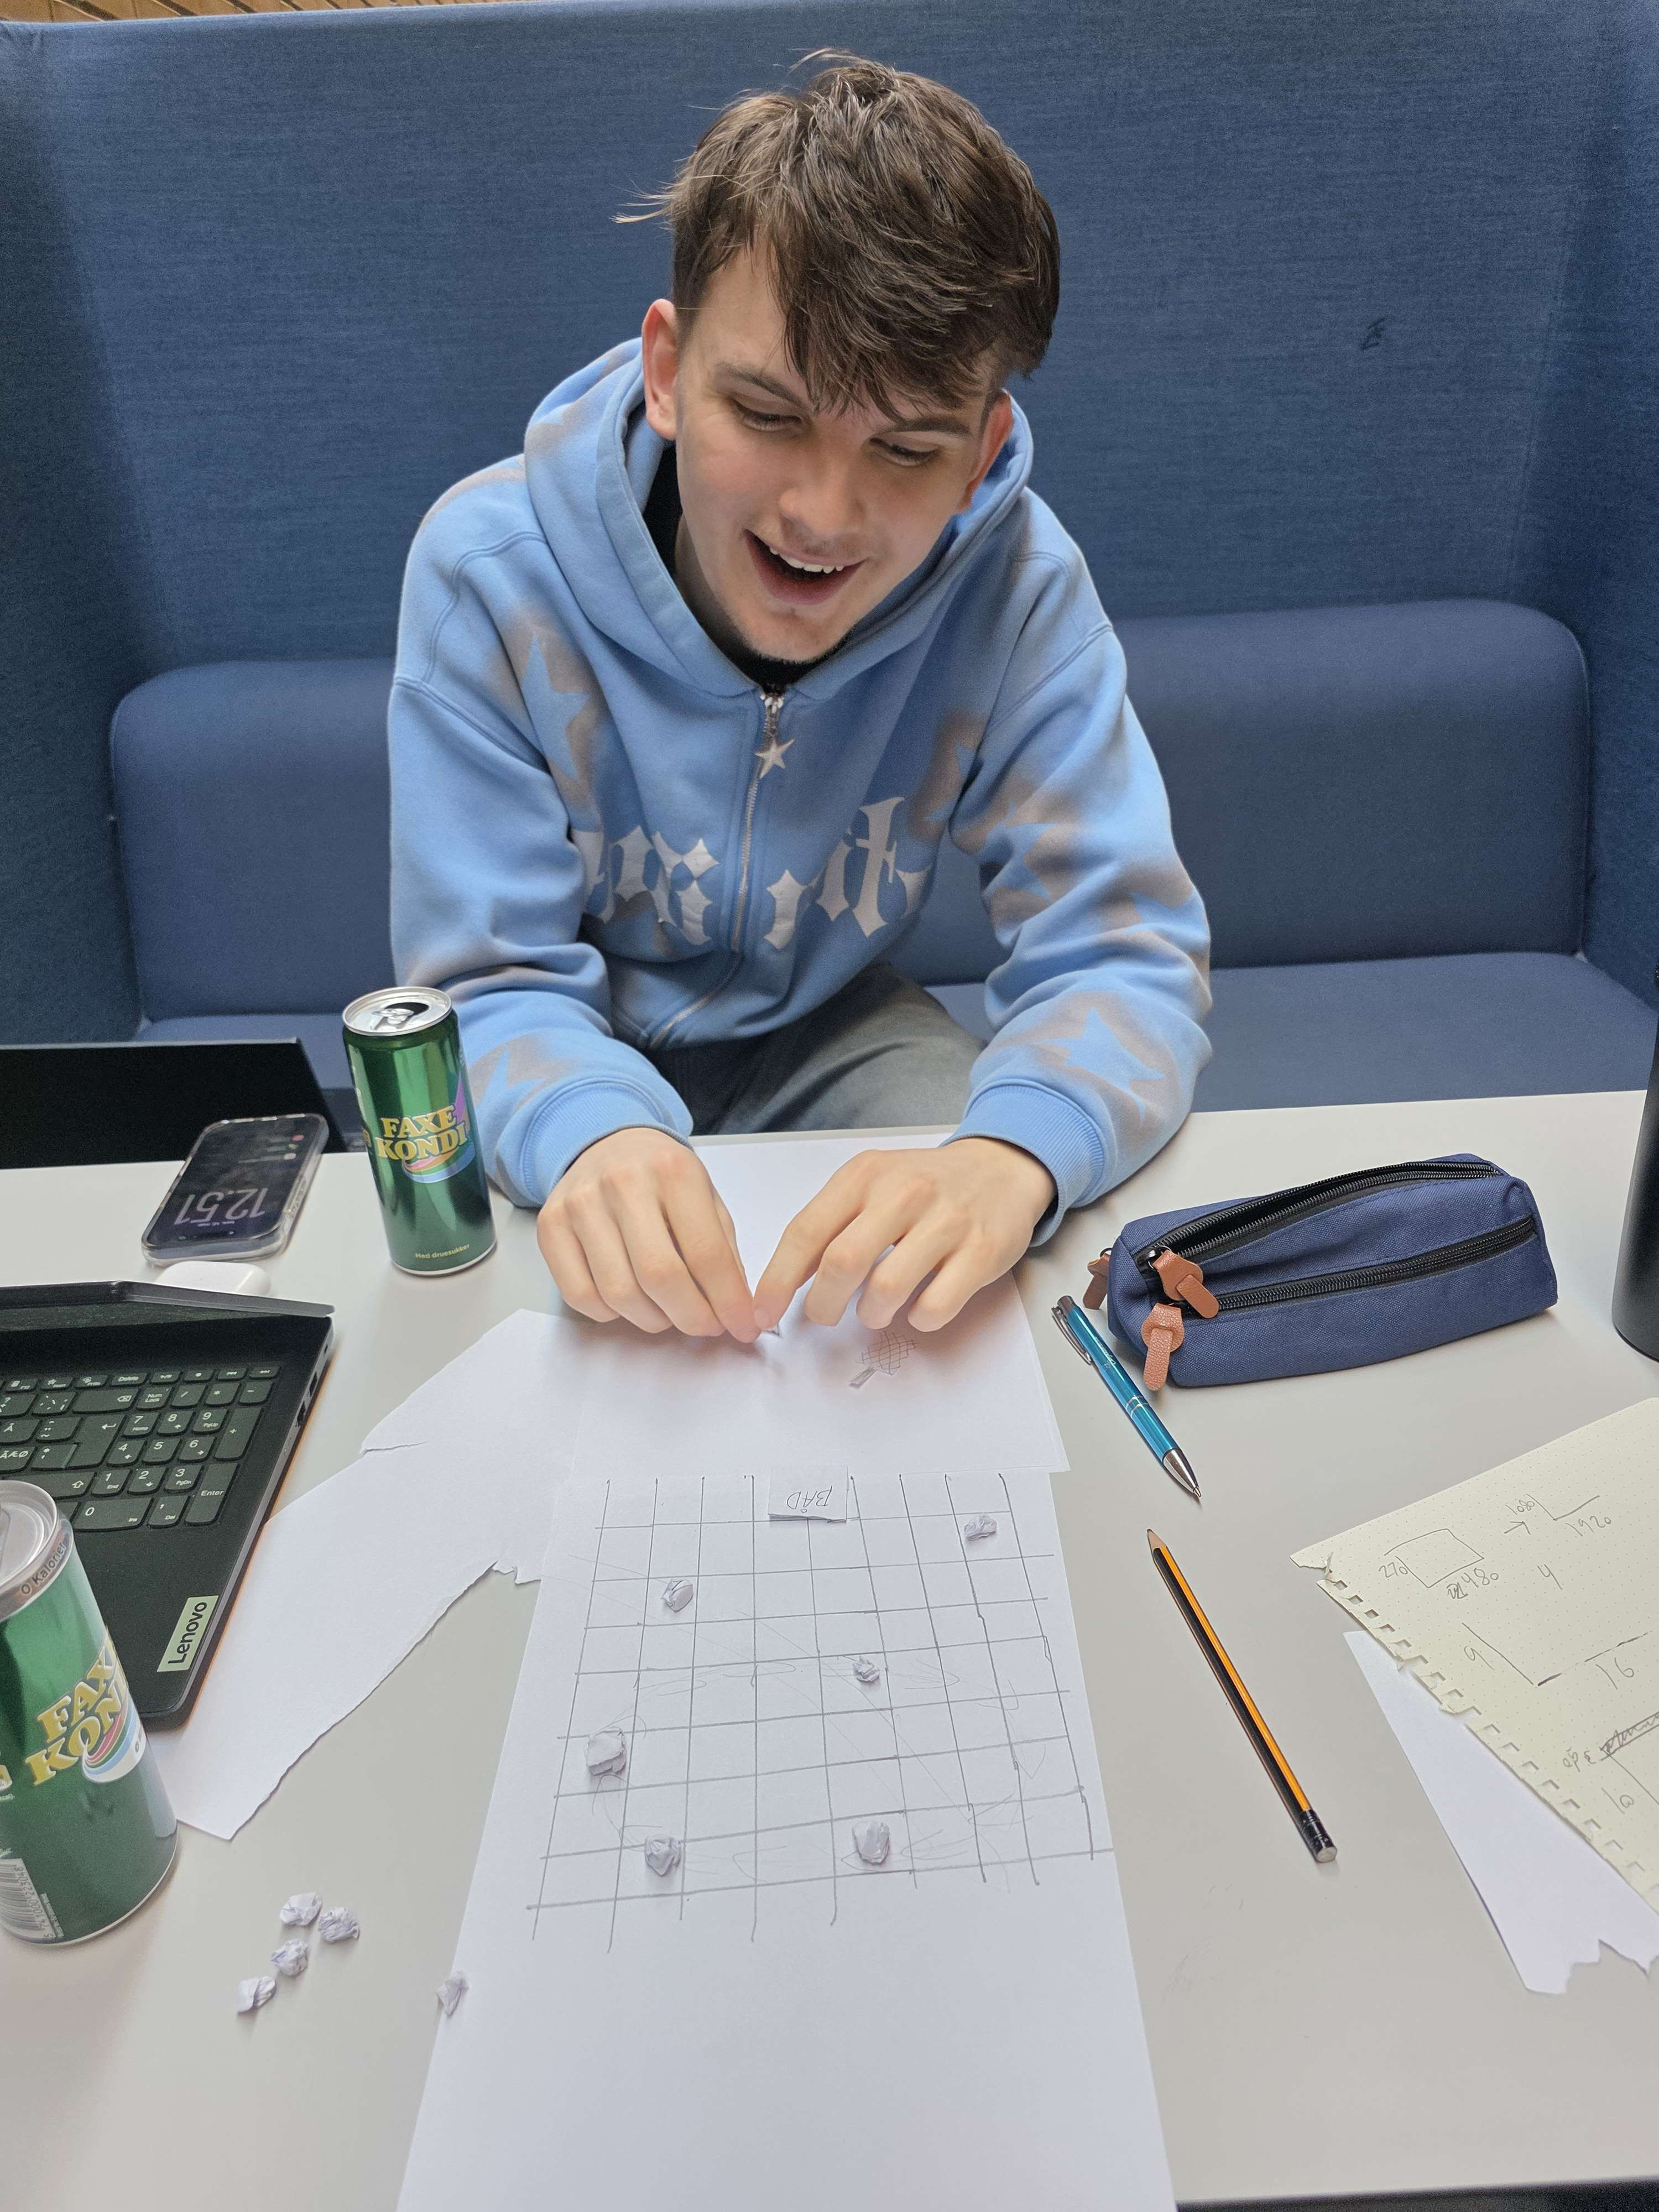
\includegraphics[width=\linewidth]{assets/paper_dummy_5.jpg}}
    % \caption{Caption e}
    \label{fig:e}
  \end{subfigure}

  \caption{Paper Dummy Testing.}
  \label{fig:main}
\end{figure}



\subsection{Spiller Movement-mechanic - white-boxing}
Det første, der implementeredes, var et rudimentært bevægelsessystem for spillerens avatar. Spilleren kan accelereres i alle hovedretningerne, altså nord, syd, øst og vest. For spilleren holdes der til enhver tid styr på spillerens hastighed $\vec{v}$ og position $\vec{OP}$ i form af vektorer. Accelerationen $\vec{a}$ er ikke bundet til spilleren, men er givet øjeblikkeligt og påvirker altså hastigheden, der igen påvirker positionen.

Når accelerationen er givet, opdateres $\vec{v}$ ved at tillægge ændringen i hastighed $\Delta \vec{v}$, der svarer til den øjeblikkelige multipliceret ændringen i tid, til den gamle hastighed $\vec{v}_0$
\begin{equation}
\vec{v}_1 = \vec{v}_0 + \Delta \vec{v} = \vec{v}_0 + \Delta t \cdot \vec{a}
\end{equation}

Herefter opdateres placeringen af spilleren $\vec{OP}$ ved at tillægge ændringen i position
\begin{equation}
\vec{OP}_1 = \vec{OP}_0 + \Delta \vec{P} = \vec{OP}_0 + \Delta t \cdot \vec{v}
\end{equation}

Således er der altså anvendt Newtonisk fysik; det er oplagt, da det er let at have med kræfterne, vi har at gøre med, mens vi har anvendt vektorregning, da vektorer har retning og størrelse, hvilket kræfter også har. Således behøver vi ikke at forholde os til x- og y-koordinaterne direkte. Udover at det er nemmere at kode, bør det også introducere færre fejl, hvor det sidste kommer slutbrugeren til gode.

Selve accelerationen er givet ved, brugerens input (dynamic) til ethvert øjeblik. Følgende keyboardtaster korresponderer til følgende
\begin{itemize}
  \item \mintinline{bash}{w} $\rightarrow$ acceleration i nordlige retning
  \item \mintinline{bash}{a} $\rightarrow$ acceleration i vestlige retning
  \item \mintinline{bash}{s} $\rightarrow$ acceleration i sydlige retning
  \item \mintinline{bash}{d} $\rightarrow$ acceleration i østlige retning
\end{itemize}

Bemærk, at dette er alle hovedretninger. Valget på netop de taster falder på, at det er etablerede konvention. Således bør det gerne være intuitivt for spilleren, og denne bør hurtigt kunne tilegne sig en evne til at bevæge sig, hvilket bør vække tilfredsstillelse hos spilleren.

Til at teste, brugte vi et simpelt mesh, fremfor en sprite, som det er i vores endelige implementering, i en simpel 2D-verden, og det virkede. Nu gennemgås implementeringsdetaljerne, for relevant Bevy-terminologi, se \autoref{par:bevy} og \autoref{subpar:ecs}. De tre systemer repræsentere hver især accelerationen, velociteten og positionen. I første omgang, eksekveres de bare per opdatering, når Bevy frigiver dataene; noget data muteres, så de kan ikke alle køre simultant.

\begin{minted}{rust}
pub fn change_player_acceleration (
    mut current_acceleration: Single<&mut crate::movement::Acceleration, (With<PlayerAvatar>, Without<crate::aim::PlayerAim>)>,
    keyboard_input: Res<ButtonInput<KeyCode>>,
    mode: Res<crate::movement::InputMode>,
    gamepad: Option<Single<&Gamepad>>,
    hand_mode: Res<crate::movement::HandMode>
  } {
    const SPEED_OF_ACCELERATION: f32 = 3000.;
    let mut weighed_direction: Vec2 = Vec2::ZERO;
    [...]
    match *mode {
      crate::movement::InputMode::Keyboard => {
        if keyboard_input.pressed(KeyCode::KeyW) {
          weighed_direction.y += 0.1;
        }
        if keyboard_input.pressed(KeyCode::KeyA) {
          weighed_direction.x -= 0.1;
        }
        if keyboard_input.pressed(KeyCode::KeyS) {
          weighed_direction.y -= 0.1;
        }
        if keyboard_input.pressed(KeyCode::KeyD) {
          weighed_direction.x += 0.1;
        }
    [...]
    current_acceleration.0 = weighed_direction.clamp_length_max(1.0) * SPEED_OF_ACCELERATION;
}
\end{minted}

Det ses, at accelerationen som udgangspunkt er 0, herefter stiger den, når spilleren trykker en af keyboardtasterne. Det ses også, at keyboardet er begrænset i modsætning til et joystick, hvor vi kan bruge den specifikke hældning; til at finde ud af den ønskede acceleration, men tilgengæld kan en lignende effekt opnås ved, at man med højere eller lavere frekvens trykker på WASD-tasterne---det vil enhver person, der har spillet Euro Truck Simulator på tastatur kunne genkende. Det fremgår af funktionens signatur, at en række andre parametre hentes, vi beskæftiger os med senere.

\begin{minted}{rust}
pub fn change_player_velocity (
    mut current_velocity: Single<&mut crate::movement::Velocity, (With<PlayerAvatar>, Without<crate::aim::PlayerAim>)>,
    current_acceleration: Single<&crate::movement::Acceleration, (With<PlayerAvatar>, Without<crate::aim::PlayerAim>)>,
    time: Res<Time>
)  {
    const FRICTION: f32 = 20.;
    const THERMAL_SPEED: f32 = 70.;
    let mut change_in_velocity: Vec2 = Vec2::ZERO;
    change_in_velocity = current_acceleration.0 * time.delta_secs();
    current_velocity.0 += change_in_velocity;
    current_velocity.0 = current_velocity.0.clamp_length_max(THERMAL_SPEED);
    if current_velocity.0.length() > 0. {
        if FRICTION * time.delta_secs() > current_velocity.0.length() {
            current_velocity.0 = Vec2::ZERO;
        }
        else {
            let direction_of_movement = current_velocity.0.clone().normalize_or_zero();
            current_velocity.0 += FRICTION * -direction_of_movement * time.delta_secs(); 
        }
    }
}
\end{minted}

Velocitet systemet er imiderltid nemmere. Her ganges accelerationen bare med deltatid og tilføjes til den nuværende velocitet. Imens anvendes en friktion, der gør, at spillerens båd efterhånden bremses; uden friktion svarer det i fysiske termer til, at der ikke sker nogen varmeudveksling mellem spillerens bådoverflade og havet---det giver ingen mening og virkede unaturligt. I høj grad har vi brugt fysikkens regler til at opnå et udgangspunkt, som vi har synes godt om, hvorefter vi har ændret på detaljerne. Det bemærkets at friktionen kun anvendes i fulde størrelse, hvis denne gange deltatid faktisk er mindre end hastigheden, ellers vil hastigheden skifte retning, og det vil den så givetvis gøre igen, konstant.

Afrundingsvist, opdateres positionen ud fra den givne velocitet. Det ses bl.a. at Bevy-queries kan være single-queries. Queries er de entiteter, der matcher vores betingelser eksempelvis skal den her indeholde et Transform-komponent og et Velocity-komponent samt være af PlayerAvatar-typen. Vi forventer kun, at spilleravataren er det, så det er en single query; hvis flere entiteter overholde denne konstruktion, kører systemtet blot ikke, og der må således være en fejl i koden.
\begin{minted}{rust}
pub fn update_player_position(
    player_query: Single<(&mut Transform, &crate::movement::Velocity), (With<PlayerAvatar>, Without<crate::aim::PlayerAim>)>,
    time: Res<Time>
) {
    let (mut position, velocity) = player_query.into_inner();
    let change_in_position = velocity.0 * time.delta_secs();
    position.translation += change_in_position.extend(0.0);
}
\end{minted}
\subsection{Skydesystem}
Skydesystemetet er lavet på en meget lig måde som for spillerens bevægelse, udover at skydesystemets konstanter gør, at spillerens sigtekorn kan bevæge sit hurtigere, men derimod en større friktion.

Det synes vi giver god mening, da præcisionbehovet er det større for sigtekornet; således er det rart, at det hviler hurtigt, mens det fysiske grundlag for, hvorfor det skal bevæge sig langsomt ikke eksistere friktionen er her helt arbitrær, men det er meget svært for et menneske, at styre noget så fint, hvis ikke det har en tophast. Denne accelerer tre gange så hurtigt som spillerens avatar, og topfarten er lidt under dobbelt så høj, mens friktionen er 14 gange større.

Selve sigtekornet er et simpelt ring mesh magen til meshet, dog mindre, vi brugte til at teste spillerens bevægelse.

Konceptet bag navigationen af sigtekornet er det samme som med spilleren, men i stedet bruges piltasterne.

\begin{minted}{rust}
  if keyboard_input.pressed(KeyCode::ArrowUp) {
    weighed_direction.y += 0.3;
  }
  if keyboard_input.pressed(KeyCode::ArrowLeft) {
    weighed_direction.x -= 0.3;
  }
  if keyboard_input.pressed(KeyCode::ArrowDown) {
    weighed_direction.y -= 0.3;
  }
  if keyboard_input.pressed(KeyCode::ArrowRight) {
    weighed_direction.x += 0.3;
  }
\end{minted}

\subsubsection{Raycasting versus faktisk simulering}\label{sec:raycast}
I spillet eksisterer der fjender, se \autoref{sec:skrald_monstre}, derfor bliver vi nødt til at have en form for hit-detektion. Umiddelbart gik vi med raycasting, hvor man skyder et ray, der basaltset er ligesom linjensparameterfremstilling, en halvlinje løber fra spillerpositionen (piben) ud mod målet og vi ser, om nogle hitboxes skæres undervejs; hvis det sker, og de ellers er de første, er det et hit, og vi traktere ved at fjerne liv fra den pågældende fjende.

Da vi afprøvede systemet virkede det dog ikke og var dårligt. Desuden renderede vi jo ikke skudene til spilleren, så det var en lose-lose-situation. Manglen på renderede skud (feedback til spilleren, hvilket spil dybestset er) kunne være afbødet ved at tilføje et flash ved piben.

Utilfredse lavede vi en ny metode, hvor vi i stedet oprettede en Bullet-entitet med en given fart og retning, herefter skulle den bare fødes, og dens position skulle opdater a la sigtekornet og spilleren, men hvor der var tale om en ikke single-query (da der jo kan være flere skud i omløb). Herefter tjekker vi bare for, om denne er indenfor hitboxen af vores mål og gøre det samme som tidligere, udover at projektilet despawnes med en Bevy-kommando.

Valget af knap til affyring af skud gik på space-knappen, da det er kutyme, at dette er en ability-tast, eller attack-tast, og tommelfingeren fint kan nå den imens resten af ens venstre hånd bruger WASD-nøglerne.

Dette system virkede dog heller ikke. Det viser sig, at fordi vi har gjort sådan, at sigtekorns-entiteten er et barn af spiller-entiteten, så eksisterer denne i et koordinatsystem, hvis position afhænger af spillerens position. Og det er ikke positionen i forhold til det globale koordinatsystem (som spilleren eksisterer i), som vi har hentet til raycastingen eller de nye beregniner, som vi har hentet men derimod dens interne koordinater. Da først vi hentede dens GlobalTransform i stedet for bare Transform, virkede systemet perfekt og det er således uvist, om raycastingen egentlig virkede. Selve raycasting-koden var lavet af AI; da det ikke er helt så ligetil at finde vektorskæringer, som vi er vant til med vores Python-matematikbiblioteker, så det var ikke smertefuldt at revidere koden. Læren må være, at man skal passe på med at stirre sig blind på problemer, der måske slet ikke er det.

Forneden ses koden, der eksplicit henter globaltransform i stedet for bare transform ved projektilets fødsel

\begin{minted}{rust}
fn shooting(
    keyboard_input: Res<ButtonInput<KeyCode>>,
    mode: Res<crate::movement::InputMode>,
    gamepad: Option<Single<&Gamepad>>,
    current_shooting_pos: Single<&GlobalTransform, (With<PlayerAim>, Without<crate::player::PlayerAvatar>)>,
    current_player_pos: Single<&Transform, (With<crate::player::PlayerAvatar>, Without<PlayerAim>)>,
    asset_server: Res<AssetServer>,
    mut commands: Commands,
) {
  [...]
  eprintln!("Shot from: {} at: {}", player_pos, target);
  commands.spawn((
      Bullet,
      Sprite::from_image(asset_server.load(PROJECTILE_PATH)),
      Transform::from_translation(bullet_origin.extend(Z_VALUE)).with_rotation(rotation),
      crate::movement::Velocity::from_vec(direction*BULLET_SPEED),
      crate::pixel_grid::PIXEL_PERFECT_LAYERS,
  ));
}
\end{minted}
\subsection{Gamepad-kompatabilitet og tilgængelighed - test II}
Da vi har at gøre med et arcade-like spil jf. \autoref{par:elevator_pitch} blev vi hurtigt enige om, at vi gerne ville implementere gamepad-kompatabilitet. Der er heldigvis indbygget support i Bevy-spilmotoren. Det er nemmere, da vægtningen i controlleren gør man mere nøgternet kan navigere, men den er også langt mere fleksibel, da der er 360-graders bevægelsesrum, og så er det dejligt analogt. I den forbindelse har vi foretaget en intern test, idet vi havde en tesis om, at højre stick skulle være til at sigte med, da dette kræver mest finmotorik (og vi er højrehåndede). Selve spillerbevægelsen er mere sekundær, da det primært handler om at skabe afstand til fjenden, så denne kan beskydes på afstand (fejlmargen er altså større), og ellers er det ``low-stakes''-dynamics som at bringe sig selve i en position, så man kan scoope skrald jf. \autoref{sec:skrald_monstre}.

Om ikke andet forventer vi, at venstrehåndede er blevet så betingede af brug af keyboard, at det nok ikke betyder det store dexterity-wise, om de sigter med piltaster eller WASD-nøgler, mens denne forskel er mere udbredt på controller. Derfor implementerede vi sammen med controller-mode også venstre- og højrehåndsmode (der kan skiftes ved at trykke left-trigger) for at finde ud af, hvor galt det ville være. Vi kunne ikke finde en population af venstrehåndede, så vi antager, at det svarer til at vi spiller på venstrehånds-mode. Og vi må bare konstatere, at det var enormt svært; så vi har valgt at inkludere dette i vores endelige produkt---så må spilleren selv om sin oplevelse. Vi har dog ikke implementeret tilsvarende for scooping-mekanikken, hvilket måske kan være en hindring.

Der kan til enhver tid kun være et inputsystem i gang ad gangen. Det skyldes, at vi frygter, såfremt begge er aktive, at begge kan risikere at accelerere spilleren samtidig, hvilket kan skabe uforudsete og uhensigtsmæssige dynamics. En controller tager til enhver tid præcedens, da det snarere er undtagelsen fremfor reglen; hvorfor bruge resurser på at forbinde en controller for så ikke at bruge den?

I princippet er gamepad-kompatabiliten agnostisk, så xbox-controller såvel som PS-dualshock-controller burde virke, men vi har kun teste på PS4-controllere, da det er det vi har haft til rådighed.

\subsection{Semi-implict Eulers metode}
På et tidspunkt, da vi brugte AI, foreslog AI, at vi brugte en semi-implicit version af Eulers metode til beregning af de nye positioner for vores mange bevægelser. Indtil da havde vi en naiv version af Eulers metode. Eulers metode er kort sagt, at du fremskriver en ny funktionsværdi ud fra en forrig funktionsværdi en trin-værdi og hældningen til den forrige funktionsværdi. Det er en numerisk metode i modsætning til eksempelvis hvis man integrerede en funktion, som man kunne gøre hvis den var kontinuer. Det vil kræve uendelig mange beregninger, og det kan vi ikke i realtid-spillogik; derfor bruger vi Eulers metode til alt fra at beregne nye hastigheder og så nye positioner. Hvor meget dette minder om ``den korrekte simulation'' afhænger af, hvor lang tid, der går imellem at vi beregner de nye udviklinger bruger dette til at opdatere vores værdier. Semi-implicit Eulers metode skal være en mere stabil og ved tilpas nok små værdier selv-korrigerende, og indebærer bare, at først opdateres accelerationen, som dernæst bruges til at opdatere hastigheden som dernæst bruges til at opdatere positionen. Det indebærer, at vi kæder systemerne sammen og tvinger dem til at køre en ad gangen efter hinanden. Bevy håndterer automatisk dataene, og har såldes prøvet på at foretage disse ændringer simultant, indtil vi eksplicit frabad det. Det betyder også denne proces i endnu højere grad har været nondeterministisk.

Forneden ses chaining i vores player-plugin, hvor bevægelsesystemerne køres per opdatering. Bemærk desuden, hvordan denne kun kører, når selve spillets hovedsløjfe er i gang (run$\_$if...).

\begin{minted}{rust}
pub fn player_movement_plugin(app: &mut App) {
    app
        .add_systems(Update, (change_player_acceleration, change_player_velocity, wave_motion, update_player_position).chain().run_if(in_state(crate::GameState::Game)));
}
\end{minted}

\subsection{Begrænsning af sigtekorn}
Et problem vi hurtigt opdagede var, at spillerens sigtekorn blev ved med at forlade spillets arena. Spilleren selv har vi tilføjet en hjemmelavet ``Nonwrappable''-attribut, der betyder, at et system, clamp$\_$to$\_$map, sikrer at denne ikke overskrider kanvasets grænser. Imidlertid kan vi ikke modificere GlobalTransform for sigtekornet pga. samme problem som med raycasting tidligere jf. \autoref{sec:raycast}. Det næstbedste er, at vi har begrænset distancen, denne må komme væk fra spilleren. Denne må ikke komme længere væk en højden af skærmen ved en 1920px1080p-opløsning. Kommer den indenfor 80 pixels af spilleren, teleporterer den om på den anden side af cirklen med en radius på 20 pixels og centrum i spilleren ved, at dens positionvektor ganges med minus 1 og derved inverteres. Præcisionen, fordi skydevinklen er så stor, bliver så lav her, at hvis den kommer så tæt på spilleren, må det være fordi denne hurtigt skal sigte et nyt sted så vi teleportere den om på cirka den anden side (man kunne måske have skåret cirklen anderledes). Såfremt det ikke er tilfældet, kan man jo ligeså let få den tilbage til der, hvor den blev teleporteret fra ved at gøre det omvendt og invertere den igen.


\subsection{Splash-screen}
Ved spillets opstart, kører to splash screens, først spillets logo dernæst Bevys. Det er selvfølgelig for at kommunikere til spilleren, at nu starter \textit{vores} spil, men det er også en hommage til spilmotoren og gerne kutyme, at man gør det. En simpel gestus, der ikke påvirker spilleren negativt, men bare forbereder denne. Havde vi haft et asset-tungt spil, kunne dette også være en måde at kamuflere asset-loading eller shader-caching i baggrunden. Splash screensne håndteres af samme state, der også markere at vi nu er i hovedsløjfen. Spillets ekskevering foreløber på følgende vis Splash1 $\rightarrow$ Splash2 $\rightarrow$ Game.

\begin{minted}{rust}
#[derive(Clone, Copy, Default, Eq, PartialEq, Debug, Hash, States)]
enum GameState {
    #[default]
    Splash1,
    Splash2,
    Menu,
    Game,
}
\end{minted}

Det ses, at Splash1 er default state. Splash-plugin'et fungerer på den simple måde, at idet gamestate bliver Splash1, hvilket det jo bliver med det samme, fødes splash-entiteten, der er sat til at despawne, når dette gamestate forlades. Desuden startes en timer a tre sekunders varighed, og når denne udløber, opdateres gamestate til næste splash, splash2, hvorefter en lignede proces begynder, der resulterer i hovedsløjfen. Plugin'et ser således ud

\begin{minted}{rust}
pub fn splash_plugin(app: &mut App) {
    app
        .add_systems(OnEnter(GameState::Splash1), splash1_setup)
        .add_systems(Update, countdown1.run_if(in_state(GameState::Splash1)))
        .add_systems(OnEnter(GameState::Splash2), splash2_setup)
        .add_systems(Update, countdown.run_if(in_state(GameState::Splash2)));
}
\end{minted}

Bemærk systemerne, der kører per opdatering. Disse tikker timeren; hvis ikke dette gøres, opdateres tiden ikke, og den afsluttes aldrig. Det er også disse systemer, der kontrollerer, om nedtællingen er færdig, og ændrer spillets state.

\subsection{Havstrømme - test III}
I et separat projekt, var det formålet at lave et simulationssystem til dette projekt, og af samme grund skal vi gøre det kort, der skulle simulere tegneserieagtige havstrømme; det slog fejl, så vi har implementerede noget mindende om i dette projekt. Kort sagt bygger det på Newtons tyngdelov med en eller flere kunstige masser og eller uden en sluthastighed (sluthastigheden opstår, når der er en friktion, der tvinger et accelererende legeme til konstant at bremse, hvorfor ændringer i hastighed (acceleration) bliver nul). Vi har udsat en population, bestående af fem mennesker, for en udvidet A/B-test. Vi gjorde det i et online-forum med følgende instruks
\begin{displayquote}
Jeg skal lave en A/B/C test. Jeg viser tre videoer. I skal angive, hvilken I synes bedst ligner havstrømme, bemærk skraldet. Skriv gerne en kommentar.
\end{displayquote}
Det skal lige siges, at tyngdefeltet kun påvirker skrald, og at skraldet har Wrappeable-typen, så de bremses ikke af grænsen. Men teleporter om på den anden side af vores arena PacMan-style. Det betyder også, at såfremt de rejser med en undvigelseshastighed, kan de undslippe vores kunstige massers tyngdefelt, men bliver stadig accelererede uden nogen sluthastighed! Det kan blive meget hurtigt. Populationen blev ikke udsat for kulminationen af denne proces men kun den spæde start heraf, dog skulle tendensen gerne fremgå.
Herefter uploadede jeg videoer af de forskellige havstrømme. Ved havstrøm A var der ingen sluthastighed og kunstig masse. Vi kaldte denne ``Det frie fald''. B var magen til på nær, at der var en sluthastighed. Vi kaldte denne ``sluthastighed''. Den sidste implementerede også sluthastighed samt flere kunstige masser. Desuden blev kvadratet af distancen mellem kunstig masse og skrald også arbitrært begrænset. Denne kvadrerede distance bliver enormt lille ved små afstande, og omvendt meget stor ved store afstande, men da vi dividerer med dette tal, bliver den resulterende kraft enormt stor, og skraldet blev trukket og fastklemt til massepunkterne---som med rigtigt tyngdekraft, bare prøv at hoppe, men vi prøver jo at emulere noget andet. Fire ud af vores fem repræsentative respondenter reagerede positivt på sidstnævnte, og vi er gået med denne implementering.

Der blev dog ikke knyttede nogle kommentarer til undersøgelsen, selvom vi opfodrede til det, hvilket kan tyde på respondenterne ikke har reflekteret mere over det eller færdiglæst vores instruks. Desuden gjorde vi det i et semi-offentligt forum, så de andre respondenterne har kunne se hinandens besvarelser, hvilket kan have gjort disse mindre selvstændige jf. The Bandwagon-effekt. 
\subsection{Skrald og monstre}\label{sec:skrald_monstre}
Skrald og monstre udgør spillets antagonister. Skrald er ikke-aktive, mens Slimey-monstrene og Trawleren, der dukker op, handler mere eller mindre.
\subsubsection{Skrald}
I spillet er der tre typer skrald, henholdsvis en dåse (Can), en vandflaske (Bottle) og en vanddunk (Water$\_$dunk). De opfører sig eksakt ens. Vi har konstanter, der kan bruges til at bestemme cirkus sammensætningen af den totale skraldemængde. Skrald fødes ved, at andre systemer skriver en besked om, at en assorteret skrald skal fødes med en given starthastighed og position. Fødselssystemet læser disse beskeder og følger trop. I systemet er førnævnte konstanter angivet. En tilfældighedsmaskine angiver et tal fra 1 til og med 100, og afhængigt af, hvad konstanterne (der tilsammen \textit{skal} give 100, ellers vil programmet crashe med vilje) er, fødes diverse konkrete typer skrald fx. kunne 50\% af skraldet fødes som flasker, da resulterer et lod mellem 1 og 51 i, at denne bliver sådan, herefter mellem 51 og 86 i dåser, og det resterende i vanddunke. Vi har med tilfældigheder at gøre, men på grund af Store Tals Lov, konvergerer sammensætningen, over et helt playthrough, mod det ønskede. Skraldet fødes pt. på den vestlige grænse, men da disse wrapper og deres retningen for deres starthastighed er tilfældig, teleporterer i hvert fald nogle af dem over på den østlige grænse. Mængden af dem, og frekvensen, hvorved de fødes tager til afhængigt af, hvilke bølge, det er, for de fødes i bølger a la Bloons TD.

Skraldet kan opsamles af en scoop-affaldsopsamler-værktøj. Det er et separat mode fra skydemodet og de er gensidigt uforenlige; spilleren må altså prioritere. Det lægger igen op til mestring, at man ved præcis, hvornår det er godt af opsamle versus selvforsvar. I spilleret er spriten ikke implementeret for opsamleren, mens en Gizmo-pakke er anvendt for at vise opsamleren hitbox i udviklingsfasen; det er også bare inkluderet i det endelige produkt som pladsholdet, det fungerer meget flydende.

\subsubsection{Slimey}
Denne først mechanic vedrørende Slimey er, at der som udgangspunkt maksimalt må være tre slimey. Når nok skrald ophober sig i en celle, er der tale om en klynge, der imploderer og bliver til Slimey, det grønne monster. Slimey er NonWrappable. Slimey jagter nådesløst spilleren, og hvert halve sekund angriber alle slimey spilleren, hvis ellers denne er tæt nok på spilleren. Fire hug fra Slimey og så er man ude. Så man har ikke løst til at blive angrebet af alle tre samtidig, mens man kan slippe afsted med at blive strejfet en enkelt gang eller to. Slimey søger lige mod spilleren og har ingen forstand for at arenaen wrapper, og kan derfor heller ikke udnytte dette; det er således også af hensyn til Slimey, at spilleren ikke bare må teleportere om på den anden side af arenaen, da Slimey ikke ville følge efter, og ej heller kan.

Slimey kan også dræbes af skud fra spilleren, men det er ikke til at sige, hvor den nye Slimey opstår; og han vil opstå, i spillets senere bølger konstant. Så der er en vis RNG forbundet med dette, hvilket selvfølgelig kan komme spilleren til skade eller til gode, men vi synes, det har en vis charme og passer ind i arkade-stillen, omend betyder det, at alle vores achievers bare må spille endnu mere for måske at være heldige. Det er klart, at der, hvor der er mere skrald, opstår han hyppigere, men det er også der, der er flere point at hente for spilleren. Det fører os til det engelske proverb

\begin{displayquote}
better the devil you know than the devil you don't
\end{displayquote}
Og det er den afvejning spilleren konstant må foretage, slår spilleren Slimey ihjel, hvilket denne vil blive nødt til, risikere den er den næste Slimey ånder spilleren lige i nakken. Omvendt er grådighed en afvejning, da spilleren må opholde sig i Slimeys arnested for at få mest muligt skrald. Desuden går pointerne blot tabt ved skraldet, der konsumeres ved Slimeys undfangst.

\subsubsection{Trawlere}
Trawleren er en slags boss. En NPC, der kommer til ved bølge 10 for at fosvare sit forurenede hav. Denne patruljerer i en sinusfunktion, og føder en masse ekstra slimeys. Den er kun til stede i ti sekunder, men har 1000 liv, så spilleren skal skyde den en del; derved lyder en række rikochetteringslyde. Lykkedes spilleren belønnes denne med 1000 ekstra point, og der lyder et stygt brag. Bemærk særligt, hvor stor trawleren er i forthold til spilleren, at der er tale om en kæmpe teknologisk forskel imellem de to; vi spiller på underdog-fortællingen. Spilleren overvældes også fuldstændig i skrald undervejs. Men går alt rigtigt, står spilleren tilbage med lidt skrald, mindre skrald og til sidste intet skrald, som en sejsherre. Lykkedes spilleren ikke med at dræbe trawleren, er der forhåbentlig så meget nysgerrighed, at denne får blod på tænderne og forsøger igen.
\subsection{Kamerabetragtninger og rendering}
Kameraet er et ortografisk kamera, da vi ikke ønsker nogen form for dybde; z-koordinaterne for vores sprites informere således bare hvilke lag, de skal renderes på. Al pixelart og logikken foregår på en 480x270 og skaleres med 4, så de præcis fylder 1920x1080. De renderes til den nærmeste heltal. Renderinglogikken er taget fra et officielt Bevy-eksempel jf. \url{https://bevy.org/examples/2d-rendering/pixel-grid-snap/}.

\subsection{Valg af stilart samt inputmetode}
Til vores spilprojekt har vi valgt at lave alt i pixel-art-stilen. Pixel-art er en moderne form for digital kunst, hvor man replikere stilen fra ældre computerspil, hvor man dengang havde markante hardwarebegrænsninger som gjorde at grafikken havde meget lavere opløsning end i dag. I moderne tid bruger spiludviklere ofte pixel-art til bevidst at skabe et retro- eller arkadeinspireret udtryk, hvilket passer godt ind i hvad vi ønsker med spillet.

Pixel-art stilen appellerer til vores målgruppe, gen Z-gymnasieelever, gennem sit retro- og arkadeinspirerede udtryk.

Vi har ligeledes valgt at udvikle spillet til controller, for at yderlige appellerer til vores målgruppe, da det er vores tesis at det taktile i særlig høj grad er ved at gøre et comeback; det ses med eksempelvis ved vinyl og Blu-Ray. Gamepad-understøttelsen giver en mere analog oplevelse af spillet.

\subsection{Pixel-art}

Til udviklingen af spillet har vi måtte producere en række grafiske elementer, som tilsammen skaber spillets visuelle udtryk. Selvom vores målgruppe ikke har et nostalgisk tilhørsforhold, der måske endda kan være kontraproduktivt, til pixel-art og datidens originale hardwarebegrænsninger, har de tilgengæld en romantisk forestilling om arkadekulturen, en anemoia (græsk ánemos "vind" og -noia "sind").\footfullcite{anemoiaGenZ}

Da spillet er udviklet i pixel-art-stilen, er alle sprites designet med lav opløsning og i et begrænset antal farver for at give spillet et retro- og arkadeinspireret udtryk. De fleste sprites er udviklet i opløsninger mellem (26 px $\times$ 16 px) og (80 px $\times$ 80 px), hvilket både understøtter pixel-art-stilen og reducerer spillets ressourceforbrug. Dette valg passer både til målgruppen (gen Z-gymnasieelever) og til spillets relativt simple gameplay, samtidig med at det gør de forskellige objekter tydelige for spilleren.

Et af de vigtigste grafiske elementer er den båd spilleren sejler rundt i. 
For at skabe en mere dynamisk oplevelse har vi designet sprites til båden i flere retninger, herunder: \textit{Vest, Syd-vest, Syd-øst, Syd, Øst, Nord-vest, Nord-øst og Nord}. Spilleren, som sidder i båden, har ligeledes separate sprites til de forskellige retninger, så karakterens orientering passer til bådens bevægelse. Dette gør animationerne mere troværdige og forbedrer spiloplevelsen. Som vist på figur \ref{fig:boat_sprites} er båden udviklet med flere retningsbestemte sprites for at skabe mere dynamiske animationer. Båd-spriten er baseret på båden vist i moodboardet (\ref{apx:moodboard}).
Båd-spritesne er udviklet i opløsningen (35 px $\times$ 35 px), hvilket gav tilstrækkelig detaljegrad til at spilleren tydeligt kan aflæse bådens retning uden at bryde med spillets simple visuelle stil.

\begin{figure}[H]
    \centering
    \fbox{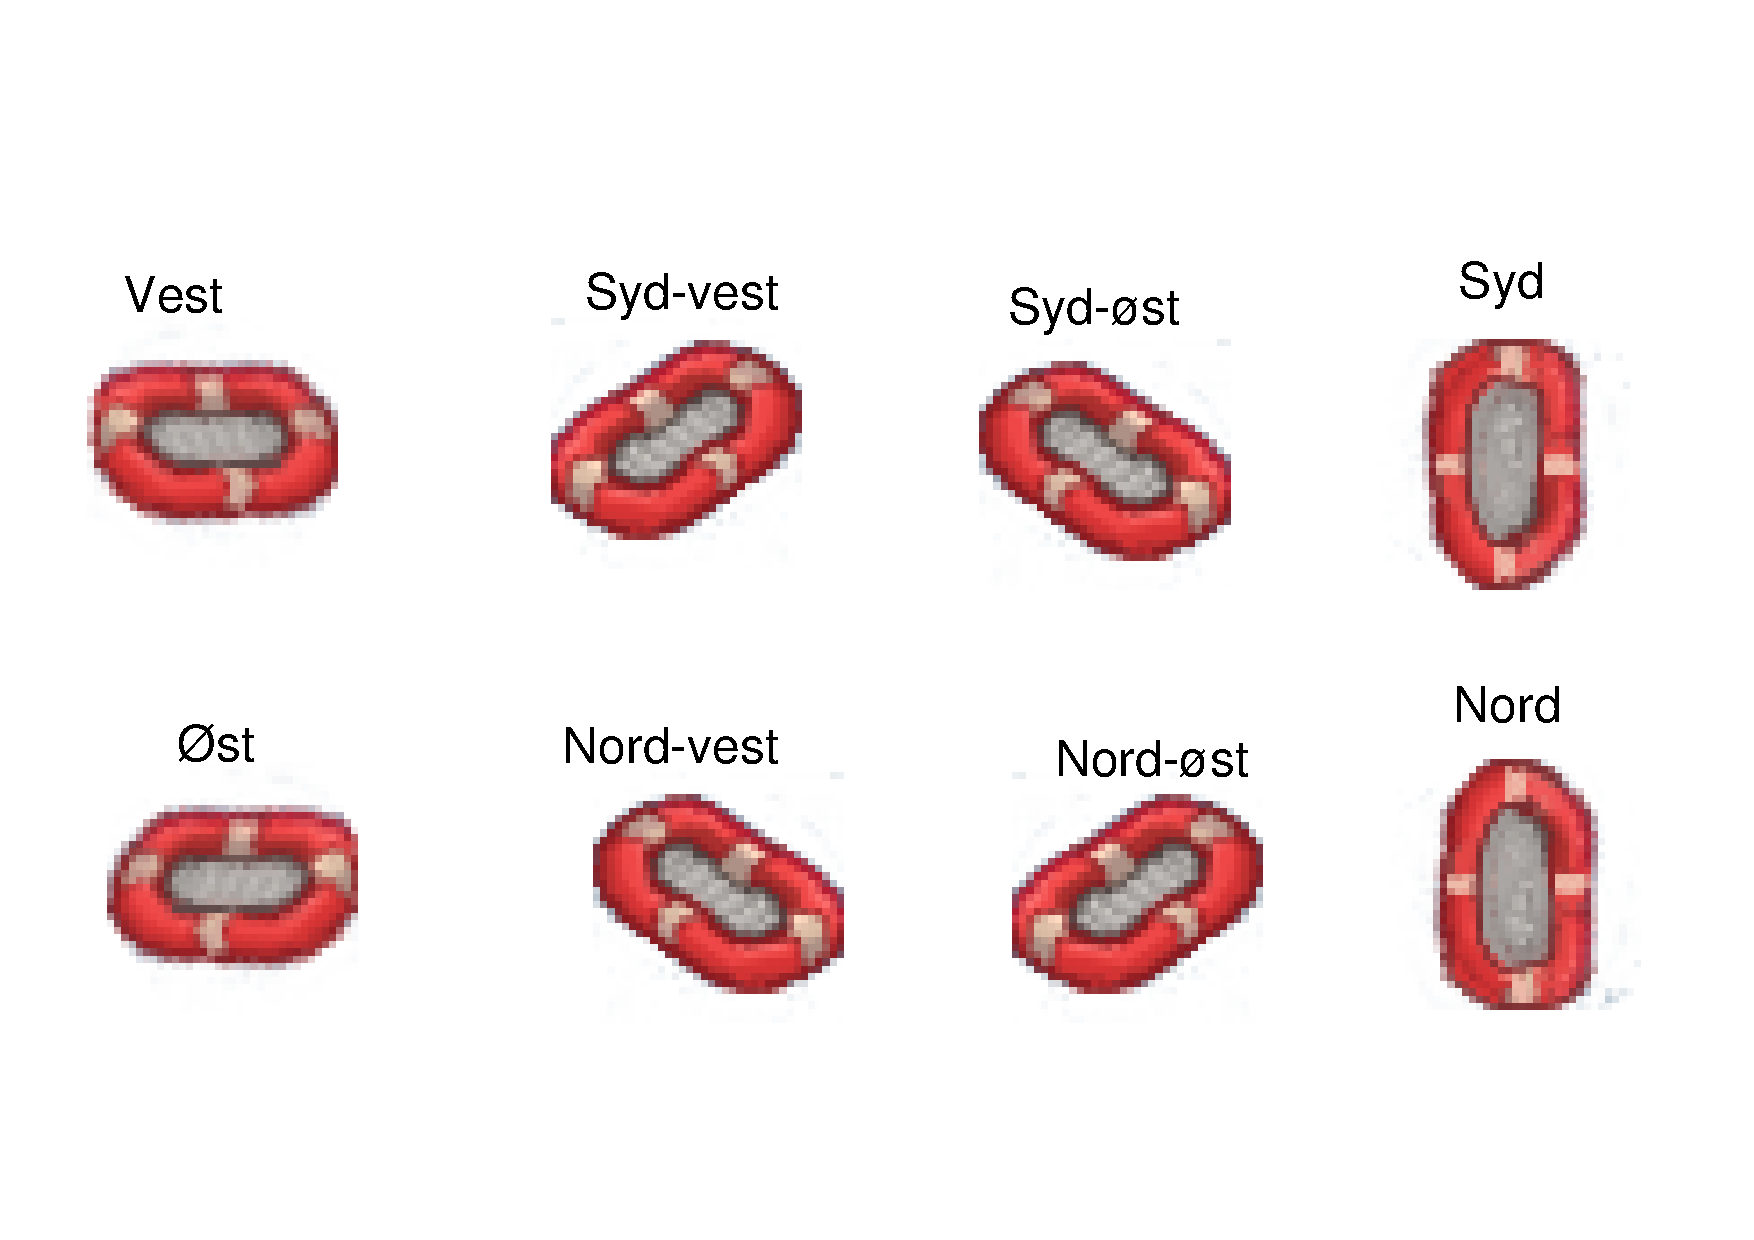
\includegraphics[width=0.7\linewidth]{appendices/sprites/sprites.pdf}}
    \caption{Sprites til spillerens båd i forskellige retninger.}
    \label{fig:boat_sprites}
\end{figure}

Motoren på båden er udviklet som separate sprites fremfor at være en fast del af både-spriten. Dette valg blev truffet ud fra både tekniske og visuelle overvejelser. Ved at opdele motoren fra resten af båden kan motor-spriten rotere uafhængigt af båd-spritens retning, hvilket gør det lettere at implementere styring og bevægelse i spillets kode. Samtidig giver det mulighed for mere fleksible animationer og et mere levende visuelt udtryk.

Derudover har vi udviklet forskellige sprites til plastikaffald, som spilleren skal samle op i løbet af spillet. Vi har valgt at fokusere på tre typer affald: en plastikvandflaske, en plastikdunk og en dåse. Disse objekter er valgt, fordi de er genkendelige former for affald, som ofte forbindes med forurening i havet. Ved at gøre affaldet tydeligt og let genkendeligt bliver spillets budskab om plastikforurening mere direkte for spilleren.


Spillet indeholder også en boss-fjende i form af et skraldemonster. Dette monster repræsenterer den ophobning af affald, som findes i havene, eksempelvis i områder som “The Great Pacific Garbage Patch”. Ligesom båden er bossen designet med sprites i flere retninger for at skabe mere flydende bevægelse og gøre mødet med bossen mere dynamisk. Bossens design adskiller sig visuelt fra de normale affaldsobjekter ved at være større og mere detaljeret, så spilleren tydeligt kan identificere den som spillets centrale udfordring. Skraldemonsteret er en videreudvikling af et design vi fandt på Pinterest\footnote{\url{https://uk.pinterest.com/pin/trash-pack-character-trashola-pixel-art--40180621656504620/}}, Vi har brugt Pinterest-designet, som ``skabelon'', og tilpasset det så det passer ind i vores spil samt tilføjet ``retninger'' så den også kan have ryggen imod skærmen. Se \autoref{fig:monster_sprites}, hvor monster-spritesne er vist.

\begin{figure}[H]
    \centering
    \fbox{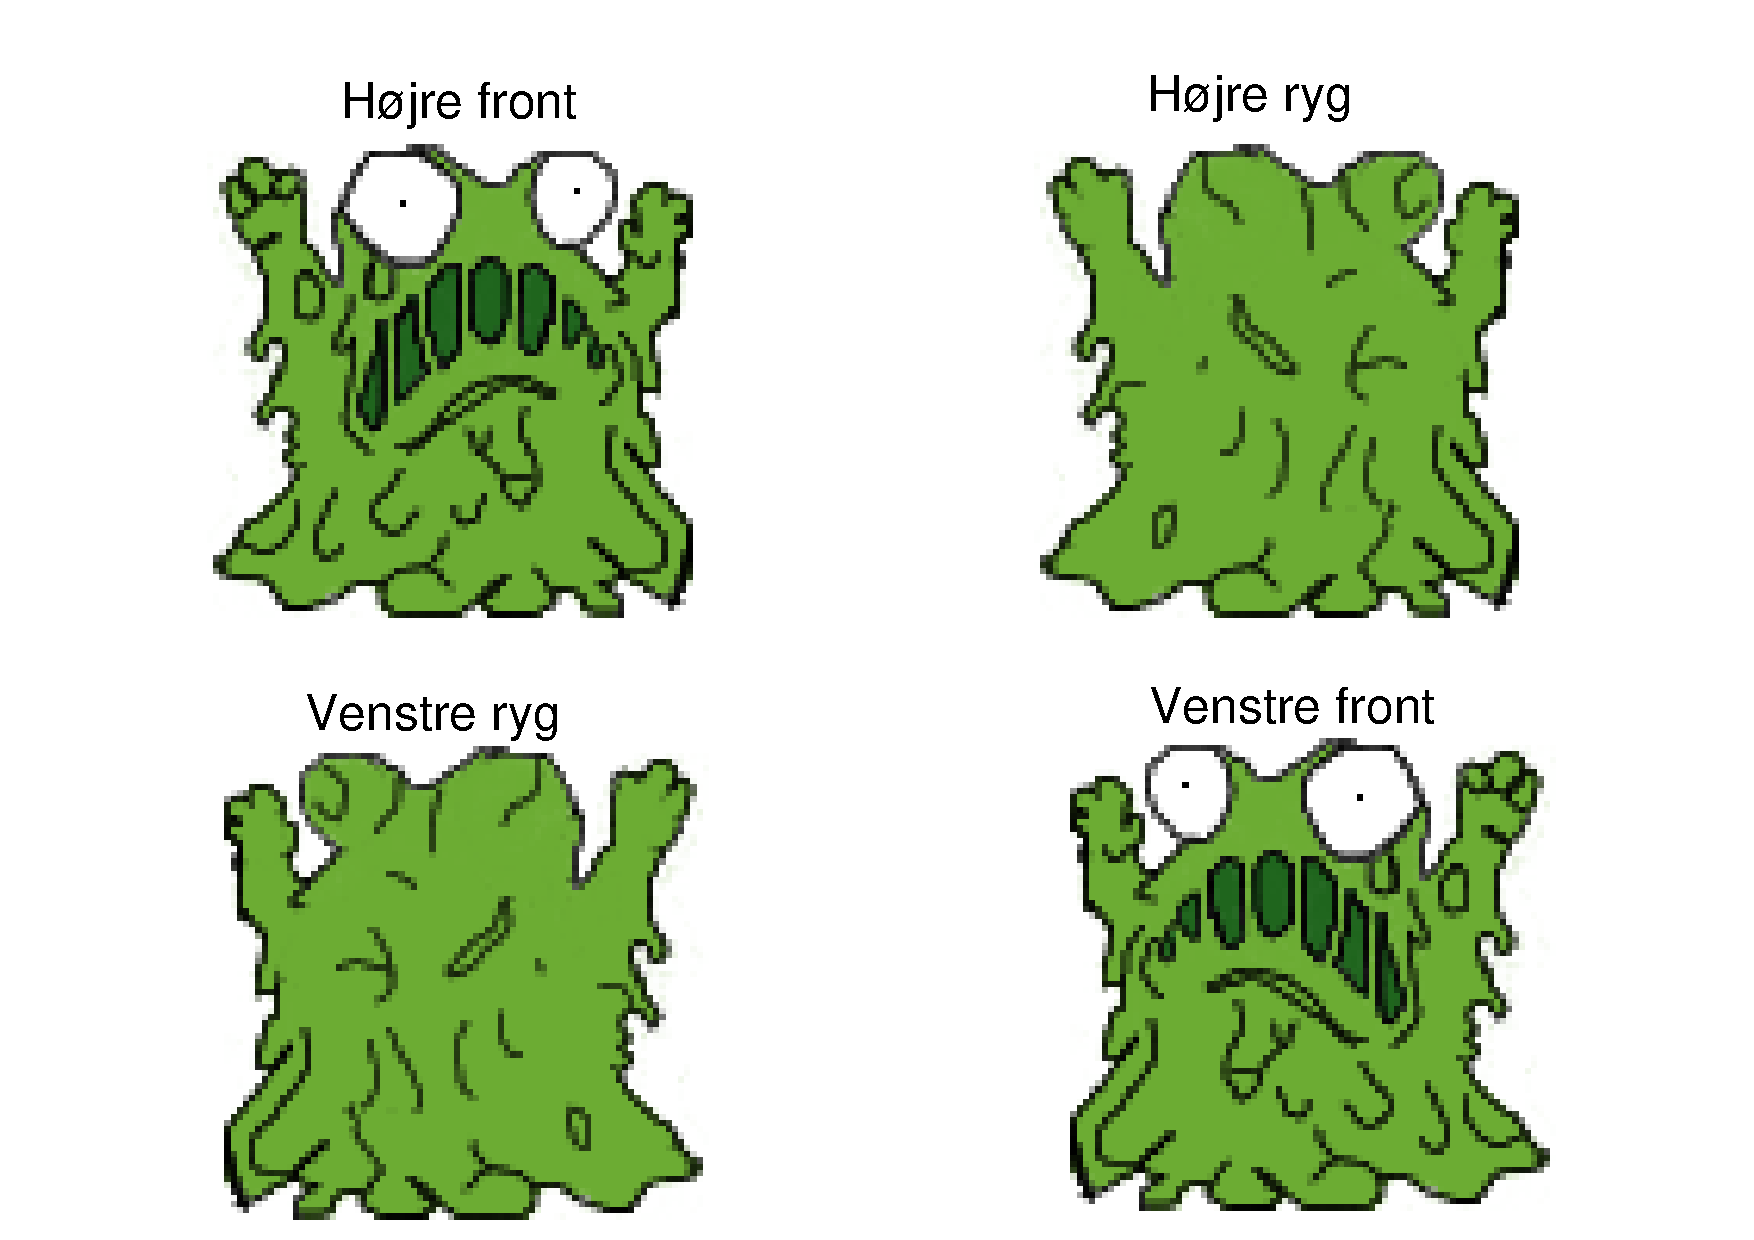
\includegraphics[width=0.7\linewidth]{appendices/sprites/monster.pdf}}
    \caption{Monster spritesne.}
    \label{fig:monster_sprites}
\end{figure}

En stor del af spillets assets er udviklet fra bunden for at sikre et ensartet visuelt udtryk og for at kunne tilpasse grafikken specifikt til målgruppen. Pixel-art-stilen blev valgt, da den både er relativt hurtig at producere inden for projektets tidsramme og samtidig appellerer til unge spillere gennem dens retro-inspirerede udtryk.
De resterednde sprites kan ses på appendiks \ref{apx:sprites}

\textbf{Trawler - test IV}\\
Trawler-asseten er blevet lavet med generativ AI (specifikt ChatGPT) Vi har valgt at bruge generativ AI til at lave denne asset, da den er ret kompliceret, og vores grafiske og kreative enskaber må siges at være begrænsede. Trawleren skal være inde for 150px $\times$ 150px og den skal være i profil. Vi har derfor promptet modellen med: \textit{``lav en oliefedtet trawler i profil i stilen pixel-art, den skal være øst-gående. 150px $\times$ 150 px''}. Promptet gav faktisk første gang to meget brugbare assets, disse fortager vi en A/B test af for at finde ud af hvilken er bedst til vores formål. Denne A/B test foretog vi uformelt i person, hvor vi spurgte 10 venner/bekendte hvilken de syntes bedst om til vores skraldeopsamlingsspil. Vi fortalte dem at trawleren skulle være ond og oliefedtet. Ud af de 10, mente 7 at trawler A var den bedste til formålet.

\begin{figure}[H]
    \centering
    \fbox{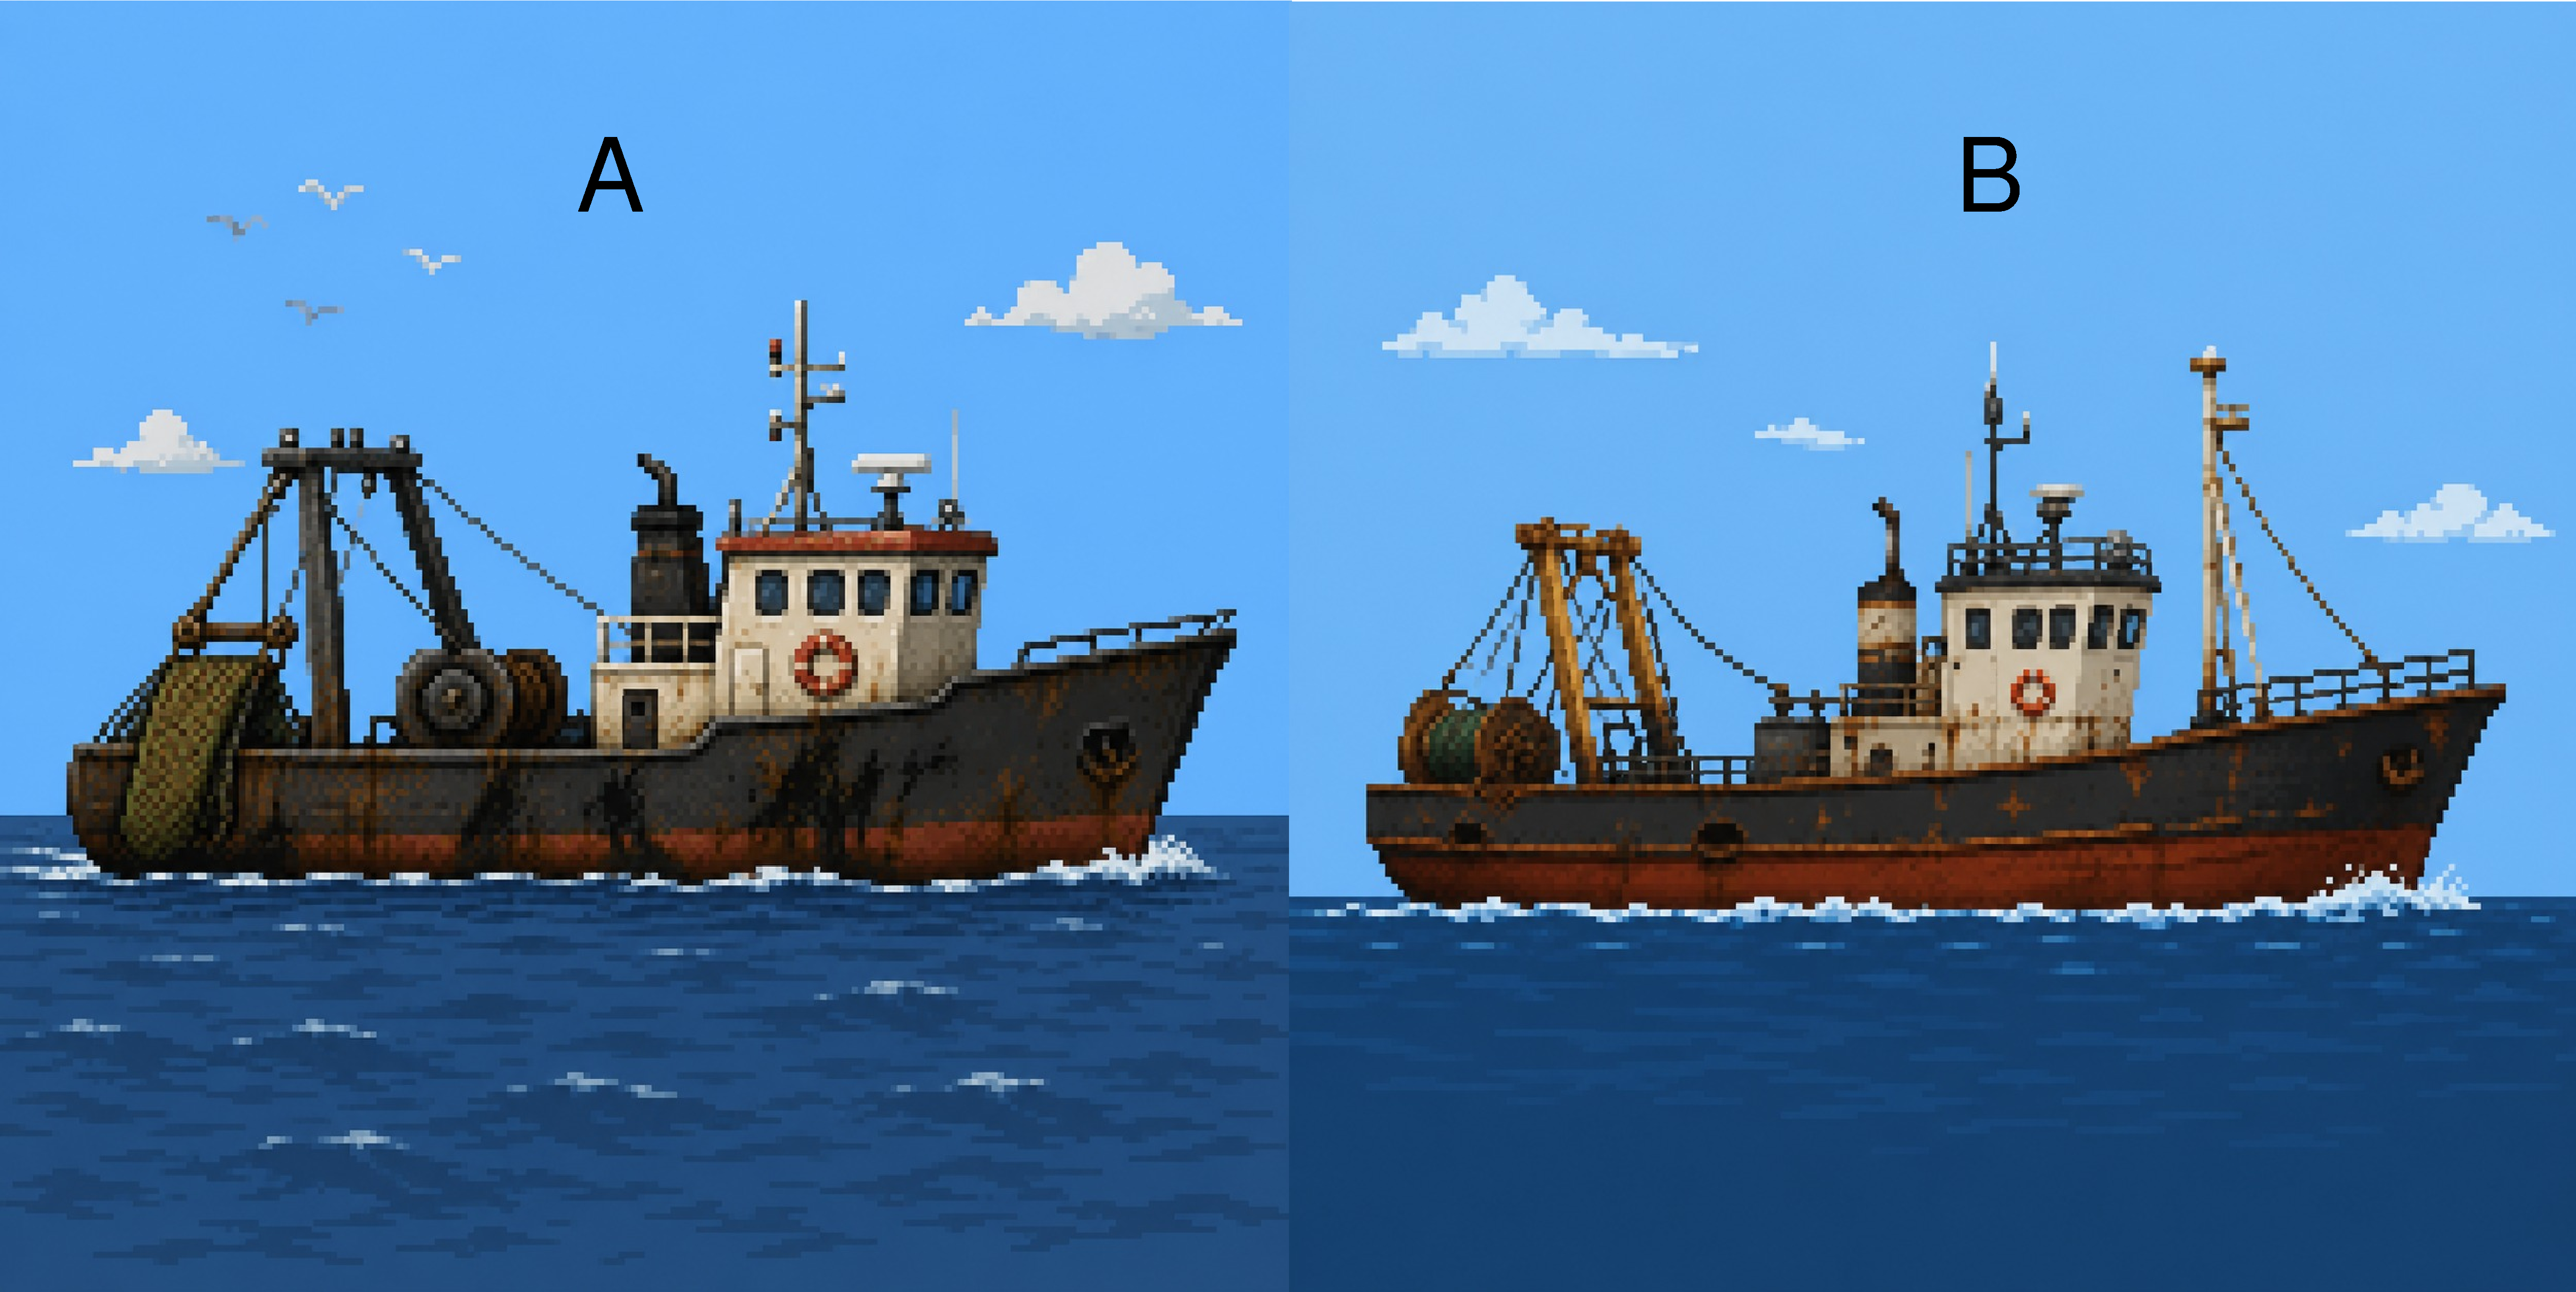
\includegraphics[width=0.7\linewidth]{assets/ai_trawler_abtest.pdf}}
    \caption{Billeder af AI-genereret trawler assets brugt til A/B test}
    \label{fig:trawler_ab_test}
\end{figure}

Nu hvor trawleren blev valgt, skal den klargøres til at indsættes i spillet. Det betyder at den skal klippes ud af baggrunden som AI-modellen ikke ville fjerne. Dette gjorde vi ved Photopea, hvor vi benyttede Magic Wand-featuren. Dernæst spejlede vi den om y-aksen for at få begge retninger.

\textbf{Outlines}\\
Vi har intentionelt designet alt det onde i spillet med sorte outlines. Dette er et stilistisk valg, som vi har truffet for at skabe en kontrast mellem det gode og det onde. Spilleren og båden har ikke nogen sort outline. Det skal få det onde til at fremstå malplaceret, mens vi implicit kommunikerer, at spilleren hører til. Den røde gummibåd skulle gerne vække minder om en helt bestemt Birthe Kjær-sang, mens rød symboliserer iver eller kærlighed.

Vi kunne have opnået en lignende effekt ved at give det gode og det onde forskellige farvepaletter.

\textbf{Fortællingen}
I spillet er vi gået med en antropocæn\footnote{At mennesket er i centrum} fortælling, selvom vi ligeså kunne have gjort spillet biocentrisk\footnote{At naturen er i centrum}, men vi vil gerne have en heroisk, menneskelig protagonist, hvor end skrøbelig han måske ser ud (humor sælger), og som måske vække minder til Happy Wheels. Men måske med en anelse af inspiration fra Project Hail Mary, lader det til at, tiden er inde for ``hoptimism'', og derfor bliver det nødt til at være et menneske, der redder dagen. Det tænker vi, ræsonnerer med vores målgruppe.

Bemærk desuden, hvordan skraldet bliver næsten klaustrofobisk, skralden er sammentømret med Slimeysne, der igen er sammentømrede med den store onde overdog---Trawleren, hvilket gerne skulle indirekte formidle spillets budskab til spilleren.

\subsection{UI-elementer - test V}
Vi har udarbejdet to UI-elementer, som viser, om spilleren enten har skyderen eller opsamleren aktiveret/deaktiveret. Spilleren har altid én af de to aktiv. Ikonerne er designet med affordance i mente. UI-elementerne har derfor relevante ikoner, som kommunikerer, at de henholdsvis er en skyder og en opsamler. Den deaktiverede er \textit{greyed out}, hvilket konventionelt betyder, at noget er deaktiveret, modsat de farvelagte, aktive knapper.
\begin{figure}[H]
  \centering
  \fbox{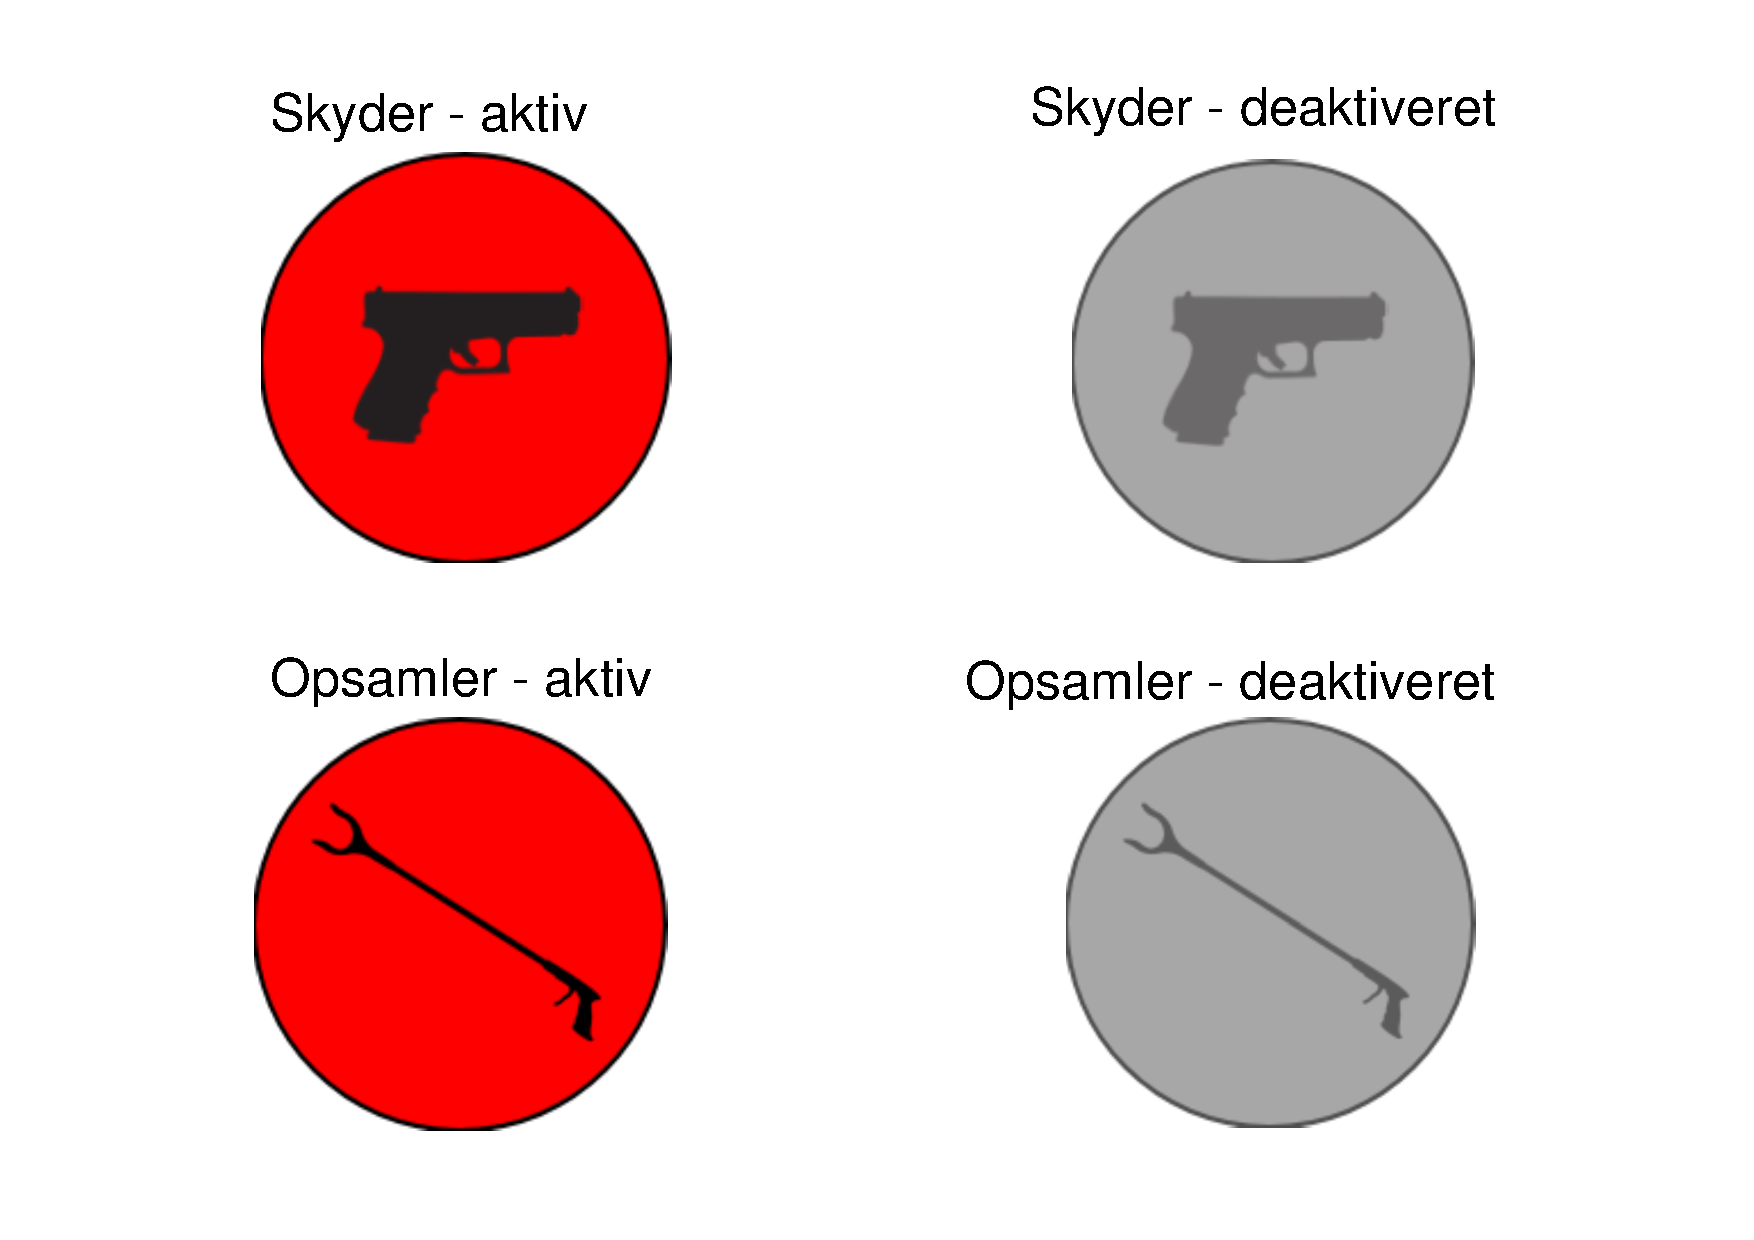
\includegraphics[width=0.5\linewidth]{assets/ui_elementer.pdf}}
  \caption{Viser to UI-elementer}
\end{figure}
Brugen af UI-elementerne er mange, og vi tester derfor placeringen af de to samt størelsen af dem. Vi har udarbejdet to gode muligheder for placeringen af UI'en. Mulighed 1 (A) er elementerne placeret nederest småt i venstre hjørne og obstruere spillet mindst muligt. Mulighed 2 (B) er elementerne meget større og tydeligere, men obstruerer skærmen mere. Vores testpersoner er som tideligere klassekammerater, og de får vist begge UI-muligheder.
\begin{figure}[H]
  \centering
  \fbox{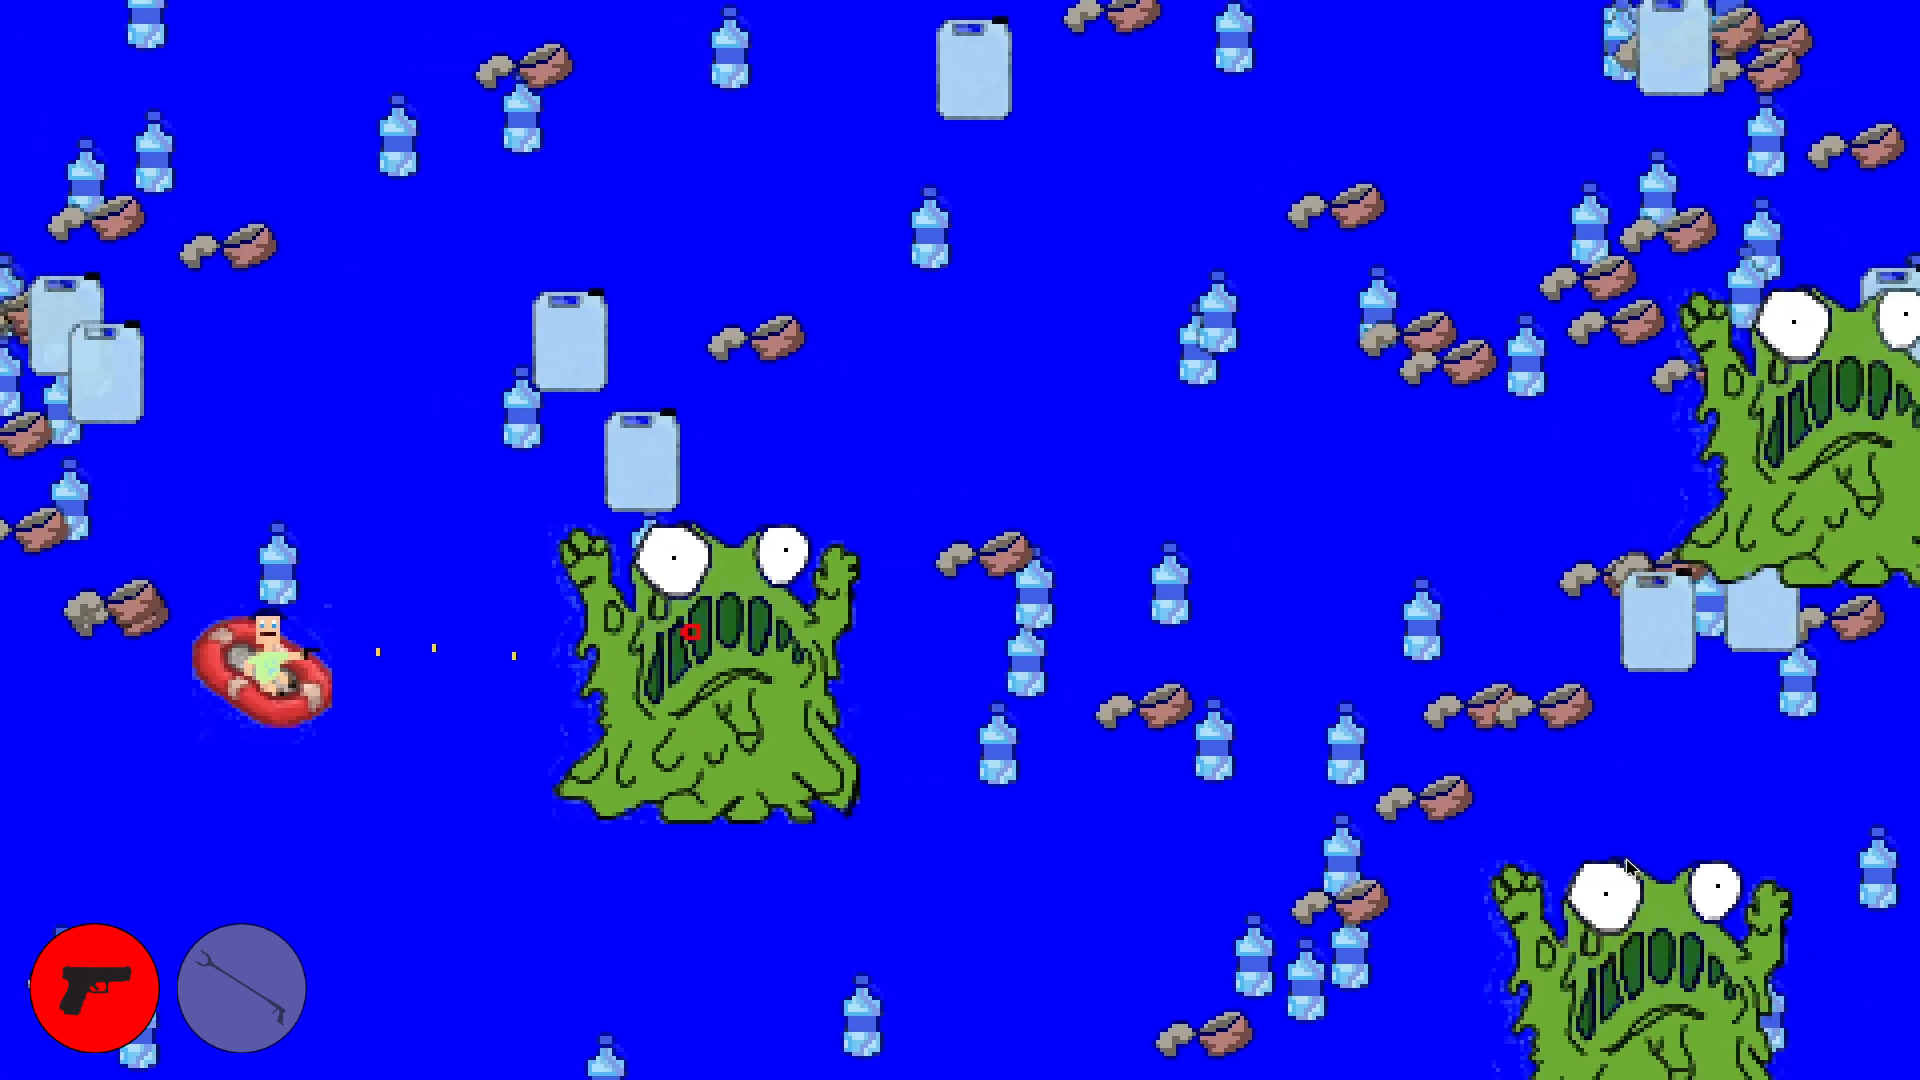
\includegraphics[width=0.5\linewidth]{assets/test_v.png}}
  \caption{Viser test V - første udgave}
\end{figure}

\begin{figure}[H]
  \centering
  \fbox{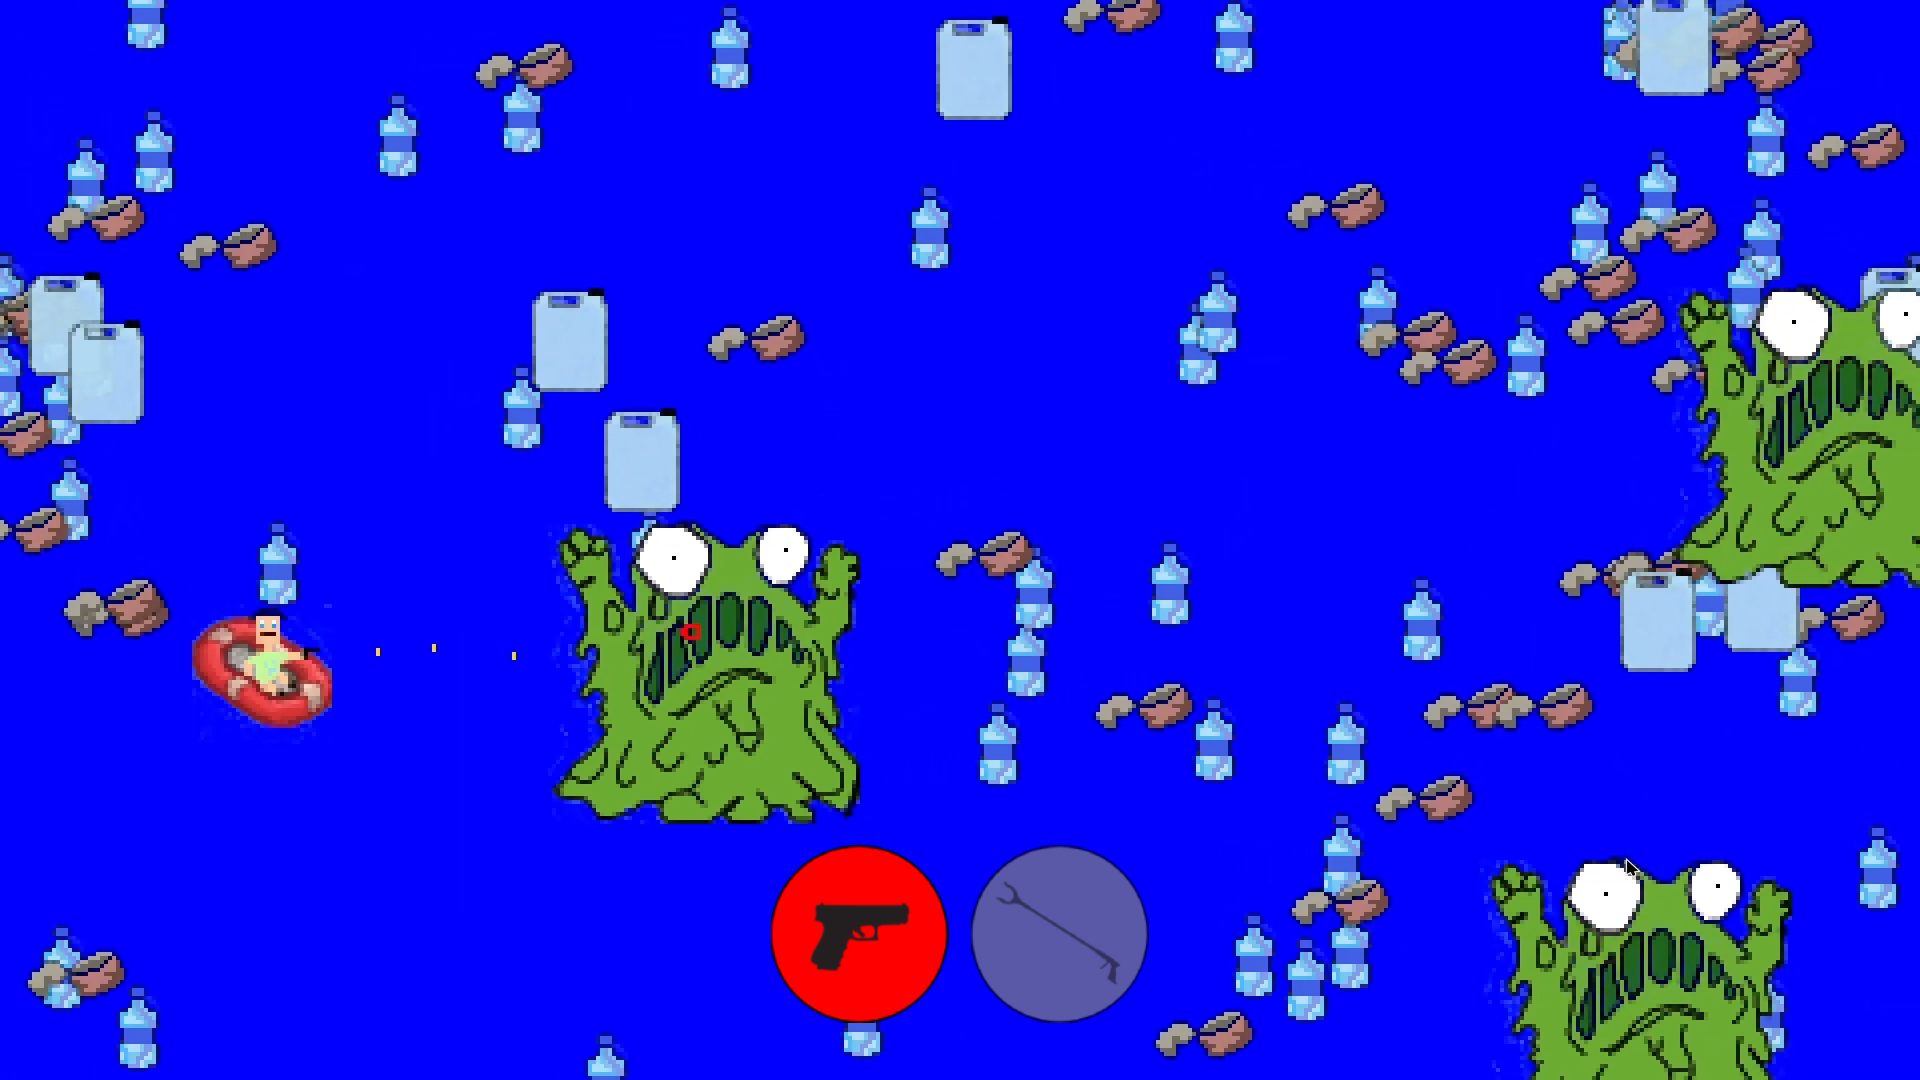
\includegraphics[width=0.5\linewidth]{assets/test_v_u2.png}}
  \caption{Viser test V - anden udgave}
\end{figure}

Denne gang har det kun været muligt at indsamle 9 resulateter fra testperosner. 7 ud af de 9 svare at mulighed A er deres preference, hovedsageligt da det obstruere mindre.

\subsection*{Spillets navn}
Spillet bærer navnet \textit{Project Plastic Waste}. Navnet er ikke blot beskrivende for spillets tema, men indeholder også en allitteration i de to P'er — \textit{Project} og \textit{Plastic} — hvilket gør navnet lettere at udtale og huske, da det falder naturligt i munden. Det kan heller ikke herske nogen tvivl om, hvad spillets omdrejningspunkt er.

\subsection{SFX og musik}
Lyddesign spiller en essentiel rolle i computerspil, da det bidrager til både stemning, feedback og spillerens oplevelse af gameplayet. I vores spil har vi arbejdet med forskellige former for SFX (sound effects) og musik for at understøtte spillets arkadeinspirerede stil og 8-bit æstetik. Den lave bitrate og retroinspirerede lydstil er valgt for at skabe en nostalgisk atmosfære, som passer til spillets visuelle udtryk og hurtige gameplay.

Til udviklingen af alle lyd-elementer har vi anvendt royalty free musik og lydeffekter fra platformene Pixabay\footnote{\url{https://pixabay.com}} og Upbeat\footnote{\url{https://upbeat.io}}. Disse valg gjorde det muligt at benytte musik og lyde uden ophavsretlige problemer, samtidig med at vi kunne finde lydmateriale, der passede til spillets tema da begge indeholder meget store biblioteker af gode lyde med mere.

Der er implementeret flere forskellige typer lydeffekter i spillet. Blandt andet anvendes skudlyde inspireret af små pistoler for at give spilleren tydelig feedback under fights. Derudover er der tilføjet lydeffekter til opsamling af skrald, så spilleren modtager øjeblikkelig lyd-respons ved succesfulde handlinger. Andre SFX omfatter lyde fra flydende skrald i havet samt lyd ved spawning af monstre, hvilket bidrager til at gøre spilverdenen mere levende og dynamisk.

Musikken er opdelt i forskellige kategorier afhængigt af spilsituationen. Den almindelige baggrundsmusik, er af tre tracks og er alle rolige og understøtter udforskning af havmiljøet, mens bossmusikken er mere intens og tempofyldt for at skabe spænding under boss fights. Derudover er der anvendt ambience-lyde fra havet, eksempelvis bølger og undervandsstemning, som hjælper med at skabe immersion og understøtter spillets miljøtema omkring havet og plastikforurening.

Ligesom pixel-art-stilen appellerer 8-bit-lydestetikken til målgruppen, gen Z-gymnasieelever, gennem \textit{anemoia}. De karakteristiske chiptune-lyde\footnote{Chiptune er en lydstil opstået fra  hardwarebegrænsningerne i tidlige spillekonsollers lydchips, kendetegnet ved  enkle, syntetiske bølgeformer.} og enkle lydeffekter er ikke noget, målgruppen selv har oplevet i deres opvækst, men de kender dem alligevel som et kulturelt og æstetisk sprog fra moderne spil og internetkulturen. Denne genkendelse uden direkte erindring skaber en særlig tiltrækningskraft, der gør lyddesignet medvirkende til at fastlægge spillet i en æstetik, som målgruppen finder autentisk og engagerende. 8-bit-lyden er således ikke blot en praktisk forenkling — det er et bevidst valg, der møder spilleren i et lyddesign, de intuitivt forbinder med netop den type arkadeinspireret gameplay, som spillet tilbyder.
